


\documentclass{abnt}			% [pnumromarab,normaltoc] Numera��o de acordo com UFPR

% Utilize a op��o normalfigtabnum para numerar as figuras e tabelas por cap�tulo
% \usepackage{hyperref}
\usepackage{bookmark}
% \usepackage{ccaption}
\usepackage[brazil]{babel}
\usepackage[latin1]{inputenc}
\usepackage{abnt-alf}
\usepackage{tabela-simbolos}
\usepackage{algorithm}
\usepackage{algorithmic}



%Package para figuras
% \usepackage{graphicx}
\usepackage{subfig}

% % % % % % % % % % % % % % % % % % % % % % % % % % % % % % % % % % % % %
% \usepackage{float}
% \usepackage{amsthm}
\usepackage{amsmath}
% \usepackage{setspace}

\makeatletter   %Para que ele entenda o @

%%%%%%%%%%%%%%%%%%%%%%%%%%%%%% Tikz commands.
\usepackage{tikz}
% \usetikzlibrary{decorations.pathmorphing,decorations.pathreplacing,decorations.shapes,arrows}
\usetikzlibrary{mindmap}
\usepackage{lscape}

% % % % % % % % % % Linhas de tablelas
\usepackage{booktabs}
\usepackage{threeparttable}

\floatstyle{boxed} \restylefloat{figure}
%%%%%%%%%%%%%%%%%%%%%%%%%%%%% PDF % % % % % % % % % % % % % % % % %
%
% \usepackage{bookmark}
%
\hypersetup{  pdfborder={0 0 0},
              pdfauthor={Wagner de Melo Reck},
              pdftitle={Algoritmos de agrupamento capacitado aplicado ao Problema de Despacho de Ordens de Servi�o}}
% \pdfinfo{
%
%    /Author (Wagner de Melo Reck)
%    /Title  (Algoritmos de agrupamento capacitado aplicado ao Problema de
% Despacho de Ordens de Servi�o)
%    /CreationDate (D:20100621095600)
%    /Subject (TCC UNIPAMPA-ALegrete)
%    /Keywords (PO, CCP)
% }

% % % % % % % % % % % % % % Renomeia
\renewcommand{\ALG@name}{ALGORITMO}
\renewcommand{\listalgorithmname}{Lista de Algoritmos}
\renewcommand{\thefigure}{\thechapter.\arabic{figure}}

\renewcommand{\resumoname}{\normalsize{RESUMO}}




\begin{document}
\renewcommand{\figurename}{FIGURA}
\renewcommand{\tablename}{TABELA}
\autor{Wagner de Melo Reck}

\titulo{Algoritmos de agrupamento capacitado aplicado ao Problema de Despacho de Ordens de Servi�o}

\orientador{Vin�cius Jacques Garcia}

\comentario{Monografia apresentada para obten��o do Grau de Bacharel em Ci�ncia da Computa��o pela Universidade Federal do Pampa.}

\local{Alegrete}

\data{Junho 2010}


% ELEMENTOS PR�-TEXTUAIS
% Capa - Obrg
\capa
% Lombada
% Folha de rosto - Obrg
\folhaderosto
\addtocounter{page}{1} %Come�a a contar aqui :)
% Errata
% Folha de aprova��o - Obrg
\begin{titlepage}
\espaco{1.1}

\begin{center}
	\Large\textbf{{Termo de Aprova��o}}
\end{center}

\vspace{0.75cm}

\begin{center}
	\large\ABNTautordata
\end{center}

\vspace{1cm}

\begin{center}
	\large\ABNTtitulodata
\end{center}

\vspace{1cm}

\noindent Disserta��o aprovada como requisito parcial para obten��o do grau de Mestre/Doutor em Minha �rea, pelo Programa de P�s-Gradua��o, Setor, Universidade Federal do Paran�, pela seguinte banca examinadora:

\setlength{\ABNTsignthickness}{0.4pt}
\setlength{\ABNTsignskip}{2cm}

\vspace{-0.5cm}
\assinatura{Prof. Dr. Meu Orientador\\Universidade Federal do Paran�}

\vspace{-0.5cm}
\assinatura{Prof. Dr. Meu Co-orientador\\Universidade Federal do Paran�}

\vspace{-0.5cm}
\assinatura{Prof. Dr. Convidado\\Universidade}

\vspace{-0.5cm}
\assinatura{Prof. Dr. Convidado \\Universidade}

\vfill

\begin{center}
	Alegrete, xx de junho de 2010
\end{center}

\end{titlepage}
% Dedicat�ria(s)
% Agradecimentos
% Ep�grafe
\pretextualchapter{~}

\vfill
\hspace{.3\textwidth}
\begin{minipage}{.6\textwidth}
	\par $\phantom{linha em branco}$
 \begin{flushright}
    \par Dedico esse trabalho � minha amada esposa, Joseane, pela paci�ncia e apoio incondicional em todos meus projetos acad�micos e pessoais.
  \end{flushright}
  \par $\phantom{linha em branco}$
 \end{minipage}

\newpage

% ******** AGRADECIMENTOS *********
% *********** OPCIONAL ************
\pretextualchapter{Agradecimentos}

\hspace{.3\textwidth}
	\par Meu primeiro agradecimento vai para minha fam�lia, sem a qual eu n�o estaria aqui vivo. Agrade�o pela paci�ncia e pela compreens�o no momentos que mais precisei (principalmente nos v�rios meses sem visit�-los), pelas palavras de apoio e conforto (\emph{``logo logo termina!''}) e claro pela sua �ndole exemplar e conhecimento �nico que pude desfrutar durante minha vida. Muito obrigado por tudo, pai, m�e e mano, os aplausos s�o para voc�s tamb�m!
    \par Acho que eu n�o estaria aqui, escrevendo esse trabalho, se n�o fosse por meu querido mestre, tutor e amigo meu professor Vin�cius Jacques Garcia, ao qual eu deve grande parte de meu conhecimento, n�o s� acad�mico mas de exemplo de pessoa. Obrigado pelas conversas amigas e paci�ncia com minha
    \par Tamb�m deve dizer que sem uma outra pessoa eu n�o estaria aqui, que dizer, eu at� estaria mas possivelmente tomando algum tarja preta ou em uma consulta num psiquiatra, o que eu quero dizer � que se eu mantenho ainda um pouco de lucidez mental � gra�as a minha amada esposa Joseane (mas chamem-na de J�). Muito obrigado pelos �timos momentos ao seu lado, por ser minha companheira nas minhas id�ias geniais (leia-se loucas), pela for�a nas aulas de c�lculo e por rir das minhas piadas (pelo menos das boas).
    \par Agrade�o ao meu gato, que tem o nome de POG mas ningu�m chama ele pelo nome, por me fazer rir quando tentava pegar o cursor do mouse.
    \par Tenho um agradecimento especial aos professores que, juntamente com meu orientador me acompanharam, no decorrer da gradua��o compartilhando seu tempo, paci�ncia e conhecimento, contribuindo muito na minha forma��o. Obrigado Amanda, Vanessa, Diego, MC(Marcelo), Alessandro, Divane, Fabiane, Fernando, Daniel, Rog�rio, Ant�nio, Vin�cius(Montagner), Deise, Eduardo.
    \par Al�m do conhecimento na gradua��o levo tamb�m a amizade e companheirismo de de v�rios colegas do nosso curso e de outros tamb�m. Obrigado pelos momentos divertidos durante os trabalhos e momentos de estudo.
    \par \#finalDoTCC



% *********** EP�GRAFE ************
% *********** OPCIONAL ************
\pretextualchapter{~}

\vfill
\hspace{.3\textwidth}
\begin{minipage}{.6\textwidth}
	\par \emph{Voc� acha que o seu problema � s�rio? | exclamou Marvin, como se estivesse se dirigindo ao novo morador de uma sepultura | E eu? O que eu fa�o se eu sou um rob� man�aco-depressivo? N�o, nem tente me responder; eu sou 50 mil vezes mais inteligente que voc� e nem eu sei a resposta. S� de tentar me colocar no seu n�vel intelectual, fico com dor de cabe�a.}
	\par Douglas Adams | O Guia do Mochileiro das Galaxias
\end{minipage}

% Resumo em l�ngua vern�cula - Obrg
\begin{resumo}
$\phantom{linha em branco}$\\
\noindent Com uma concorr�ncia cada vez maior, as empresas devem tornar suas opera��es cada vez mais enxutas para evitar gastos desnecess�rios. Para empresas que atendem clientes distribu�dos por uma cidade, esses atendimentos devem ser feitos de maneira otimizada, evitando desperd�cios, tanto financeiros quanto de tempo, com deslocamentos desnecess�rios. Para evitar tais deslocamentos, o despacho dos atendimentos para as equipes  deve levar em considera��o a localiza��o dos atendimentos e o tempo necess�rio para executar tal atendimento. Para representar isso, podemos olhar esse problema como um problema de agrupamento capacitado, onde desejamos associar os atendimentos com as equipes de modo que todos atendimentos associados a uma equipe estejam pr�ximos uns dos outros e que seja poss�vel de executar todos eles dentro de sua jornada de trabalho.

\noindent Este trabalho faz um estudo de alguns m�todos heur�sticos cl�ssicos na literatura para o problema de agrupamento capacitado e de busca local aplicados ao problema de despacho de ordens de servi�o (PDOS), tratando tamb�m sobre algumas caracter�sticas das inst�ncias como a capacidade total excedente e a dispers�o dos atendimentos no espa�o. Al�m disso, n�s desenvolvemos um pequena altera��o em um dos m�todos j� existentes, de modo que o m�todo resultante conseguiu produzir solu��es melhores que que obtidas com o m�todo original para a grande maioria das inst�ncias.\\
$\phantom{linha em branco}$\\
\begin{espacosimples}
Palavras-chave: PO; Heur�sticas; PAC, Agrupamento.
\end{espacosimples}
\end{resumo}

% *********** ABSTRACT ************
\begin{abstract}
$\phantom{linha em branco}$\\
\noindent With competition increasing, companies must make their operations more lean to avoid unnecessary expenses. For companies that serve customers spread over a city, these services must be made optimally, avoiding waste, both financial and time, with unnecessary travels. To avoid such displacement, dispatching of calls for the teams must take into account the location of call in space and time required to perform such call. To represent this, we can look at this problem as a capacitated clustering problem, where we want to associate the calls with the teams so that all calls associated with a team are close to each other, reducing the distance between the calls, and that it is possible they all run within team's workday.

\noindent This work is a study of some classical heuristics methods in the literature for the clustering problem and local search apllyed to the service order dispatch problem (SODP), dealing also with some characteristics of the instances as the total capacity surplus and dispersion of care in space. In addition, we developed a small change in one of the existing methods, so that the resulting method could produce better solutions than that obtained with the original method to the vast majority of instances.\\
$\phantom{linha em branco}$\\
\begin{espacosimples}
Key-words: OR; Heuristic; CCP, Clustering;
\end{espacosimples}
\end{abstract}
% Resumo em l�ngua estrangeira - Obrg
% Lista de ilustra��es
\listadefiguras
% Lista de tabelas
\listadetabelas
% Lista de abreviaturas e siglas
\listadesiglas
% Lista de s�mbolos
% Sum�rio - Obrg
\sumario

% ELEMENTOS TEXTUAIS
% Introdu��o Obrg
\chapter*{Introdu��o}
Em alguns setores de empresas, para efetuar o atendimento a um cliente, elas
devem deslocar um funcion�rio (ou uma equipe deles) da sua base de opera��es at�
a casa do cliente para executar o servi�o.
Isso ocorre principalmente em empresas que prestam algum tipo de servi�o de
atendimento domiciliar aos clientes, como por exemplo empresas de entrega de
correspond�ncia, provedores de internet no que diz respeito a suporte aos
clientes e companhias de distribui��o de energia el�trica tamb�m referente aos
suporte a clientes.
% Esse ultimo cen�rio que esse trabalho toma emprestado para os estudos de caso.

Esses tipos de atendimentos aos clientes s�o chamados de ordens de servi�o (OS)\sigla{OS} {Ordem de servi�o},
 podendo ter outros nomes conforme a �rea de atua��o da empresa, mas sempre com
 o intuito de registrar que a empresa deve fazer um atendimento a um determinado
cliente.
Cada OS contem alguns dados b�sicos como localiza��o do atendimento e tempo
previsto de atendimento. Trataremos aqui a localiza��o como um ponto no espa�o
$\Re^{2}$ e o tempo como a demanda de tempo que a OS levar� para ser atendida.

Como medida de deslocamento apenas consideraremos apenas a dist�ncia euclidiana
entre os pontos, pois algumas inst�ncias reais se fossem representadas com a
dist�ncia real que a equipe percorreria, iria demandar um mapa completo da
localidade e m�os das ruas, o que nem sempre � dispon�vel.

Nesse cen�rio de estudo tomamos algumas premissas como v�lidas:
\begin{itemize}
 \item Uma OS deve ser atendida por um funcion�rio/equipe;
 \item N�o levamos em considera��o agendamentos de hor�rios, apenas que todas as OS devem ser executas;
 \item Uma OS possui um tempo que a equipe levar� para exuta-la;
 \item Uma equipe consegue executar todas as OS atribuidas a ela no tempo estimado e predefinido de cada uma delas;
 \item O tempo de atendimento de todas as ordens atribuidas a uma equipe n�o deve ultrapassarem sua jornada de trabalho que � pr�viamente estipulada;
 \item As ordens s�o as de apenas um dia. As que entrarem durante o atendimento ficam agendadas o pr�ximo dia.
 \item N�o ser� considerado o tempo de deslocamento entre os atendimentos das OS.
\end{itemize}

Essas premissas definem o PDOS \sigla{PDOS} {Problema de Despacho de Ordens de Servi�o}, onde
devemos associar todas OS as equipes de modo que uma OS seja atendida por uma, e n�o mais que uma, equipe.
Minimizar o deslocamento entre os atendimentos � algo desej�vel para as empresas, pois diminui os custos e o tempo de deslocamento entre os atendimentos pela menor dist�ncia percorrida.

Ao designar um conjunto de OS a uma equipe, deve-se levar em considera��o a  carga hor�ria de cada mesma e a demanda de tempo que cada OS do conjunto.
 Isso por si s� pode ser visto como um Problema da Mochila, o que j� n�o � um problema de solu��o trivial.

Ao atribuir as OS levando em considera��o apenas a carga hor�ria da equipe e o tempo demandado pelas OS pode nos levar a solu��es como as apresentadas na figura \ref{FigDemandaCapacidade}, onde temos 3 equipes atendendo um total de 15 atendimentos.
\begin{figure}
 \begin{center}
  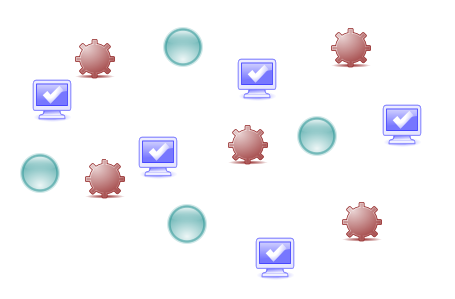
\includegraphics[scale=0.5]{./images/DemandasCapacidade.png}
 % DemandasCapacidade.png: 455x299 pixel, 96dpi, 12.04x7.91 cm, bb=0 0 341 224
  \end{center}
\caption{\label{FigDemandaCapacidade}Aloca��o de OS apenas pelas Demandas e
Capacidades }
\end{figure}

� poss�vel perceber que os atendimentos de cada equipe encontram-se
dispersos, necessitando um maior deslcomento das equipes de um atendimento a
outro do que se os atendimentos estivessem agrupados mais pr�ximos.

Um problema que engloba essas caracter�sticas apresentadas � o  CCP \sigla{CCP} {Problema de Agrupamento Capacitado - Capacitated Clustering Problem}, cl�ssico na literatura e tamb�m conhecido como (CPMP) \sigla {CPMP}{Problema das P-Medianas Capacitado - Capacitated P-Medians Problem}.
 Na figura \ref{FigCCPIntro} temos um exemplo de como as ordens de servi�o poderiam estar associadas �s equipes.

� poss�vel perceber que ainda assim n�o foi poss�vel atribuir as OS de modo que todas OS de de uma equipe fique pr�ximas de uma OS escolhida como centro.
 Isso � devido as restri��es de capacidade das equipes e demandas das OS.

\begin{figure}
 \begin{center}
  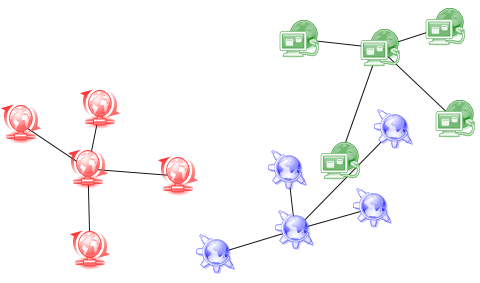
\includegraphics[scale=0.5]{./images/CCPIntro.png}
 % DemandasCapacidade.png: 455x299 pixel, 96dpi, 12.04x7.91 cm, bb=0 0 341 224
  \end{center}
\caption{\label{FigCCPIntro} Poss�vel atribui��o das Mesmas OS segundo CCP }
\end{figure}

As inst�ncias in�ditas desse problema foram retiradas de ordens de atendimento
de um concession�ria de distribui��o de energia el�trica e tiveram que ter a
capacidade de atendimento normalisadas para ser poss�vel gerar solu��es v�lidas
do problema. Esse fato ocorre pelo fato de encontrar uma solu��o � necess�rio
existir uma folga entre das demandas e a capacidade. � frente neste trabalho ser�
apresentado um estudo sobre essas folgas.

Nesse trabalho n�o trataremos da gera��o de rotas entre os atendimentos, mas
esse problema j� foi tratado na literatura como o CTSP \sigla{CTSP} {Problema do Caixeiro Viajante
Agrupado - Clustered Travel Salesman Problem}, onde desejamos entrar os menor ciclo Hamiltoniano nos pontos, sendo que os pontos
dos agrupamentos devem ser visitados em sequ�ncia \cite{jeanCTSP-Genetic}.

 %Inclui arquivo introducao.tex
% Desenvolvimento - Obrg
\chapter{Problema de Agrupamento}

Agrupamento n�o apenas expressa o ato de separar dados em grupos, mas separa-los de modo que os elementos dos grupos resultantes tenham alguma, ou mais de uma, caracter�stica em comum entre si.
 Segundo Lorena e Furtado \cite{lorena2001constructive} ``problemas de
 agrupamento
 geralmente aparecem em classifica��o de dados para algum prop�sito como armazenar e
 recuperar ou analisar dados. Todo algoritmo de agrupamento tentar� determinar algum
 agrupamento inerente ou natural nos dados, usando medidas de dist�ncia ou similaridade entre os dados.''.

Um exemplo bem simples de agrupamento seria o ato de separar poucas frutas de apar�ncia boa das de
 apar�ncia n�o t�o boa dado uma medida de apar�ncia.
 Para esse exemplo, um ser humano conseguiria executar a tarefa de forma
competitiva com um algoritmo, mas quando inclu�mos um grande de dados de entrada
e desejamos que sejam levadas em considera��o outras medidas ou outras
restri��es (ex. dividir em 10 grupos sendo 5 de frutas melhores al�m dos objetos
de cada grupo sejam de cores e tamanhos semelhantes), os algoritmos de
agrupamento podem chegar a uma solu��o muito melhor em menor tempo.

Dentre as aplica��es pr�ticas podemos destacar o uso de agrupamentos para data
mining,
 processamento de imagens, procura por padr�es,
Redu��o de cores de imagens, localiza��o de facilidades, reconhecimento de
padr�es, aloca��o de tarefas a m�quinas

Os problemas de particionamento podem ser organizados segundo a taxonomia
mostrada por \cite{jain1999data} reproduzida na figura \ref{clusterTaxonomy}.
\begin{figure}
 \begin{center}
\begin{tikzpicture}[mindmap, scale=0.9]
\begin{scope}[mindmap, concept color=orange, text=white]
\node [concept] {Agrupamentos} [clockwise from=-45]
  child{node [concept]{Hier�rquico} [clockwise from=0]
    child{node [concept]{Link Simples}}
    child{node [concept]{Link Completo}}
  }
  child{node [concept]{Particionado}
    child{node [concept]{Erro dos Quadrados}[clockwise from=-45]
          child{node [concept]{K-Means}}
    }
    child{node [concept]{Grafo te�rico}}
    child{node [concept]{Solu��o de Mistura} [clockwise from=-135]
        child{node [concept]{Expectativa de Maximiza��o}}
    }
    child{node [concept]{M�todo de Busca}}
  }
;
\end{scope}
\end{tikzpicture}
\caption[Taxonomia dos problemas de agrupamento]
   {\label{clusterTaxonomy}Taxonomia para os problemas de agrupamento}
\end{center}
\end{figure}
Os problemas de particionamento, que ser�o aprofundados nesse trabalho, s�o
problemas onde � desejado descobrir parti��es nos conjuntos de dados de modo que
cada parti��o contenha apenas elementos similares entre si.

A escala de dificuldade de resolver do problema de particionamento, ser vista pela express�o de distintas parti��es $p$ existente em $n$ pontos,$N(n,p)$,
definida por \cite{liu1968cl}:
\begin{equation}
 N(p,n) = \frac{1}{p!}\sum_{i=0}^{p}(-1)^{p-1}\binom{p}{i}i^{n}
\end{equation}

Ahmadi e Osman apresentam em \cite{ahmadi2004density} um exemplo do resultado da
computa��o dessa express�o para uma inst�ncia com 50 pontos, o resultado pode
ser visto na imagem \ref{ahmadiCalc}.
\begin{figure}
 \begin{center}
 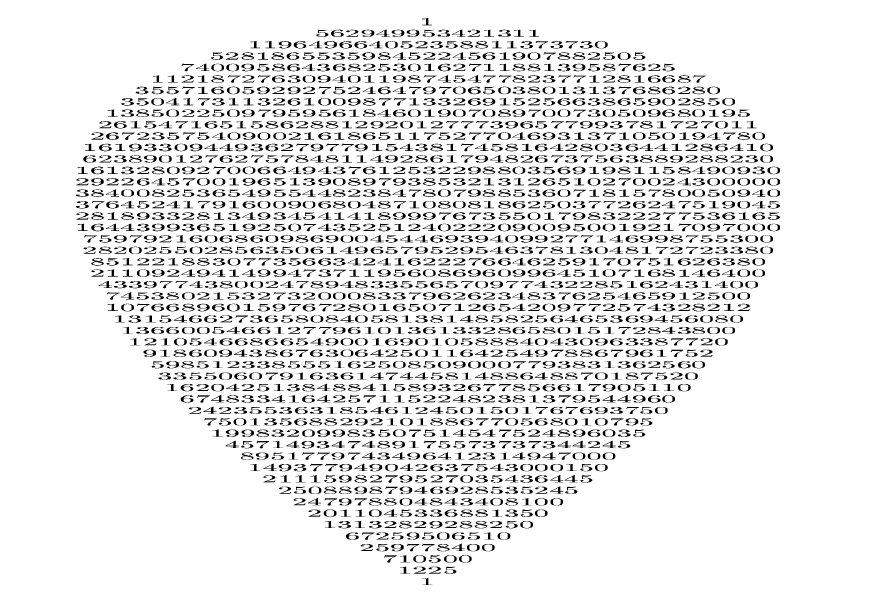
\includegraphics[scale=0.3]{./images/Ahmadi_Values_N_n_p.png}
 % Ahmadi_Values_N_n_p.png: 880x606 pixel, 96dpi, 23.28x16.03 cm, bb=0 0 660 454
\end{center}
\caption[Valores para N(n,p)]{\label{ahmadiCalc}Valores para N(n, p). No topo p
= 1 e na base p = 50.}
\end{figure}

Pode ser observado que mesmo para inst�ncias n�o t�o grandes, o espa�o
de busca � gigante. Quando consideramos inst�ncias maiores, como as resolvidas
por Taillard \cite{taillard2003heuristic}, onde s�o tratados 2863
pontos, o espa�o de busca cresce ainda mais. O uso de m�todos exatos �
proibitivo pelo tempo computacional que seria necess�rio para essas inst�ncias
maiores, e sendo esses problema da classe NP-Completo \cite{garey1979computers}
n�o existe um algoritmo que resolva de forma exata em tempo polinomial, o que
resta � o uso de m�todos heur�sticos e h�bridos.
Outro fato sobre esses dados � que a ocorr�ncia de mais agrupamentos poss�veis,
ocorra com $p=16$, o que vem a mostrar que o problema � assim�trico em rela��o
a p.

Os problemas de agrupamentos por particionamento est�o, do ponto de vista de
complexidade, entre os problemas combinatoriais mais dif�ceis de serem
resolvidos \cite{ahmadi2004density}

Quando temos um conjunto de pontos no espa�o ($\Re^{2}$ por exemplo) e
desejamos agrupar os pontos pela sua  localiza��o, podemos utilizar como
medida de dispers�o dos grupos a dist�ncia dos pontos em rela��o ao centroide
calculado pelos pontos do agrupamento. Esse � tamb�m conhecido como Problema das
K-M�dias (K-Means) apresentado por \cite{macqueen1966some}

O problema das P-Medianas � uma varia��o do problema das K-M�dias, com a diferen�a de utilizar uma mediana (um dos indiv�duos) como refer�ncia para medi��o das similaridades dos pontos de cada um dos agrupamentos.

Acrescentando a restri��o de capacidade aos agrupamentos, temos o problemas das P-Medianas Capacitado ou tamb�m tratado na literatura por CCP.

\section{CCP - Problema de Agrupamento Capacitado}
Como j� apresentado anteriormente, o CCP tem por objectivo agrupar indiv�duos de modo a maximizar as similaridades entre entre todos indiv�duos de um agrupamento e a mediana do pr�prio agrupamento. Para o caso dos indiv�duos serem representados por pontos no $\Re^{2}$, temos como similaridade o posicionamento dos mesmos no plano, a qual � medida pela dist�ncia entre eles. Na Fig. \ref{fig:Exemplo-CCP} � apresentado um exemplo de uma poss�vel solu��o do CCP dado um conjunto de pontos.

\begin{figure}
\begin{centering}
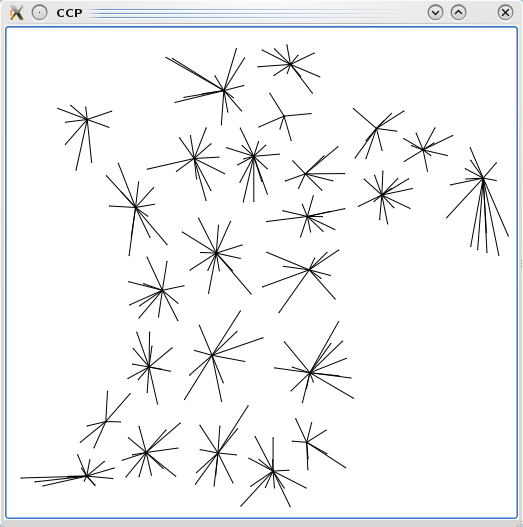
\includegraphics[scale=0.5]{../TCC-I/imagens/cluster_Density_SJC4a.png}
\par\end{centering}
\caption{\label{fig:Exemplo-CCP}Exemplo de uma solu��o do CCP}
\end{figure}

O problema de agrupamento capacitado pode ser visto como: dado um conjunto
$I$ de $n$ indiv�duos com suas respectivas demandas $d_{i}\: i\in I$,
� desejado agrupar os $n$ pontos em $p$ agrupamentos, onde a soma
das demandas em cada agrupamento deve ser menor que a capacidade total
do agrupamento, $Q_{j},\:\forall j\in P$, sendo $P$ o conjunto de
agrupamentos, e � desejado minimizar as dissimilaridades entre uma mediana do
agrupamento, para isso possu�mos uma matriz $c_{IxI}$ com as dist�ncias entre todos os pontos. O problema pode ser representado pela seguinte formula��o matem�tica \cite{ahmadi2004density}:

\begin{equation}
Min\;\sum_{i\in P}\sum_{j\in I}c_{ij}x_{ij}\label{eq:obj_CCP}\end{equation}
Sujeito �:
\begin{equation}
\sum_{j\in p}x_{ij}=1,\;\forall i\in I\label{eq:1Cluster_CCP}\end{equation}
\begin{equation}
\sum_{j\in P}y_{j}=p\label{eq:numClusters_CCP}\end{equation}
\begin{equation}
x_{ij}\leq y_{j,\;}\forall i\in I,\:\forall j\in P\label{eq:mustAssign_CCP}\end{equation}
\begin{equation}
\sum_{i\in I}q_{i}x_{ij}\leq Q_{j},\;\forall j\in P\label{eq:capacity_CCP}\end{equation}
\begin{equation}
x_{ij},\: y_{j}\in\{0,1\},\;\forall i\in I,\;\forall j\in P\label{eq:sets_CCP}\end{equation}

Em (\ref{eq:obj_CCP}), temos a fun��o objetivo que minimiza a dist�ncia
entre os componentes de cada agrupamento com a mediana do agrupamento. A medida $c_{ij}$, do ponto $i$ at� o ponto $j$ (mediana do agrupamento), somente � considerada
se o ponto $i$ est� associado ao agrupamento $j$ pela vari�vel bin�ria $x_{ij}$, sendo $x_{ij}=1$ caso o ponto $i$ esteja associado ao agrupamento $j$ e $0$ caso contr�rio. A restri��o (\ref{eq:1Cluster_CCP}) indica que cada ponto deve estar associado a um agrupamento. J� (\ref{eq:numClusters_CCP}) indica que devem existir $p$ agrupamentos. Os indiv�duos somente devem ser associados a agrupamentos existentes (\ref{eq:mustAssign_CCP}), sendo $y_{j}$ o conjunto de pontos escolhidos como medianas, sendo $y_{j}$ igual a 1 se $j$ for uma mediana e 0 caso contr�rio. Para garantir que a capacidade $Q_{j}$ de um agrupamento $j$ n�o ser� ultrapassado, � colocada a restri��o (\ref{eq:capacity_CCP}). A �ltima restri��o, (\ref{eq:sets_CCP}), especifica as vari�veis inteiras de decis�o.

Quando temos o valor de capacidade dos agrupamentos homog�neo, ou
seja, o valor de $Q_{j}=Q_{i}\:,\forall j\: e\:\forall i\in P$, podemos
dizer que esse � um problema das $p-medianas$ capacitado.

\subsection{CCCP}\sigla{CCCP}{Problema de Agrupamento Centrado Capacitado - Capacitated Centred Clustering Problem}
Um outro problema de agrupamento foi proposto por Negreiro e Palhano\cite{negreiros2006capacitated}
� o CCCP (Capacitated Centred Clustering Problem - Problema de agrupamento
centrado capacitado) onde os agrupamentos passam a ter seu centro
n�o necessariamente em um ponto (mediana), mas no centroide calculado
entre os pontos pertencentes a cada agrupamento.

s�o propostas 2 varia��es do problema, $p-CCCP$, onde � dado o n�mero
de agrupamentos que se deseja encontrar, e $g-CCCP$ (generic - CCCP)
que se deseja encontrar o menor n�mero de agrupamentos para atender
a todas demandas, sendo a fun��o objetivo em ambas a minimiza��o das
dissimilaridades entre os componentes de cada agrupamento.

Na figura \ref{fig:CCCP} � apresentada a visualiza��o de uma solu��o
para o problema $CCCP$.

%
\begin{figure}
\begin{centering}
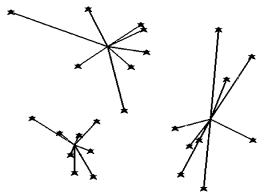
\includegraphics{../TCC-I/imagens/CCCP}
\par\end{centering}

\caption{\label{fig:CCCP}Uma solu��o para CCCP \cite{negreiros2006capacitated}}
\end{figure}


A primeira, $p-CCCP$, possui o n�mero fixo de agrupamentos que se
deseja encontrar e a segunda varia��o, $g-CCCP$, assume que para
cada novo agrupamento adicionado, � acrescentado um valor de penaliza��o
na fun��o objetivo, levando a minimiza��o de agrupamentos. A defini��o
para o $p-CCCP$ �:

\begin{equation}
min\sum_{i\in I}\sum_{j\in P}\parallel a_{i}-\overline{g_{j}}\parallel^{2}x_{ij}\label{eq:obj_CCCP}\end{equation}
Sujeito �,

\begin{equation}
\sum_{j\in P}x_{ij}=1,\;\forall i\in I,\label{eq:1Cluster_CCCP}\end{equation}
\begin{equation}
\sum_{i\in I}x_{ij}=n_{j},\;\forall j\in P,\label{eq:nPerCluster_CCCP}\end{equation}
\begin{equation}
\sum_{i\in I}a_{i}x_{ij}=n_{j}\overline{g_{j}},\;\forall j\in P,\label{eq:centroid_CCCP}\end{equation}
\begin{equation}
\sum_{i\in I}q_{i}x_{ij}\leq Q_{j},\;\forall j\in P,\label{eq:capacity_CCCP}\end{equation}
\begin{equation}
a_{i}\in\Re^{l},\;\overline{g_{j}}\in\Re^{l},\; n_{j}\in N,\; x_{ij}\in\{0,1\},\;\;\forall i\in I,\;\forall j\in P,\label{eq:sets_CCCP}\end{equation}

onde, $\overline{g_{j}}$ � o centroide do agrupamento $j$, $n_{j}$o
n�mero de indiv�duos associados ao agrupamento $j$, $a_{i}$a posi��o
do indiv�duo $i$ no espa�o $\Re^{l}$, $q_{i}$a demanda do indiv�duo
$i$, $Q_{j}$ a capacidade de cada agrupamento, $I$ o conjunto de
indiv�duos e $P$ o conjunto de agrupamentos.

A fun��o objetivo (\ref{eq:obj_CCCP}) tem como diferencial em rela��o
ao problema cl�ssico $CCP$, o fato das similaridades serem medidas
em rela��o a todos pontos do agrupamento at� seu centroide, o qual
n�o � necessariamente um indiv�duo. A eq. (\ref{eq:1Cluster_CCCP})
indica que um indiv�duo somente pode estar associado a um agrupamento,
e a restri��o (\ref{eq:nPerCluster_CCCP}) associa a $n_{j}$o n�mero
de indiv�duos no agrupamento $j$. Em (\ref{eq:centroid_CCCP}) �
definido todos os centroides dos respectivos agrupamentos e em (\ref{eq:capacity_CCCP})
� colocado que cada agrupamento n�o pode maior demanda dos indiv�duos
que sua pr�pria capacidade. A ultima restri��o (\ref{eq:sets_CCCP})
indica o dom�nio das vari�veis do problema.

No $g-CCCP$ o n�mero de agrupamentos n�o � definido a priori, mas
tem um limitante inferior dado por $\lceil\sum_{i\in I}q_{i}/\sum_{j\in P}Q_{j}\rceil$.
Esse problema a seguinte formula��o:
% \begin{singlespace}
\begin{eqnarray}
Min &\;& \left(F\sum_{j\in P}z_{j}\right)+\sum_{j\in P}\left(\sum_{i\in I}\parallel a_{i}-\overline{g_{j}}\parallel^{2}x_{ij}\right)\label{eq:obj_g-CCCP} \\
Sujeito\;A,&& \\
\sum_{j\in P}x_{ij} &=& 1,\;\forall i\in I,\label{eq:1Cluster_g-CCCP} \\
\sum_{i\in I}a_{i}x_{ij} &=&  \overline{g_{j}}\left(\sum_{i\in I}x_{ij}\right),\;\forall j\in P,\label{eq:centroid_g-CCCP} \\
\sum_{i\in I}q_{i}x_{ij} &\leq& Q_{j}z_{j},\;\forall j\in P,\label{eq:capacity_g-CCCP}  \\
\overline{g_{j}}&\in&\Re^{l},\: z_{j},\: x_{ij}\in\{0,1\},\;\forall i\in I,\forall j\in P,\label{eq:sets_g-CCCP}
\end{eqnarray}
% \end{singlespace}
onde, $z_{j}=1$ se o agrupamento $j$ est� aberto (em uso), $0$
caso contr�rio, $Q_{j}$ a capacidade do agrupamento $j$, $q_{i}$a
demanda o indiv�duo $i$, $\overline{g_{j}}$ o centroide do agrupamento
$j$. $F$ � o custo fixo para abrir um novo agrupamento.

A fun��o objetivo (\ref{eq:obj_g-CCCP}) minimiza as dissimilaridades
entre os integrantes de um mesmo agrupamento al�m do n�mero total
de agrupamentos abertos. A eq. (\ref{eq:1Cluster_g-CCCP}) define
que um indiv�duo somente pode estar associado a um agrupamento, (\ref{eq:centroid_g-CCCP})
encontra o centroide de cada agrupamento e (\ref{eq:capacity_g-CCCP})
garante que a capacidade dos agrupamentos n�o sejam ultrapassados.
As ultimas restri��es (\ref{eq:sets_g-CCCP}) especificam as vari�veis
de decis�o.


\section{M�todos de resolu��o}
Devido a caracter�sticas como o tamanho de espa�o de busca, a resolu��o de problemas de particionamento utilizando m�todos exatos ou de otimiza��o como \emph{branch and bound} s�o inefetivos em inst�ncias maiores \cite{osman1994capacitated}.

Para obter solu��es em tempos computacionais vi�veis (por exemplo no caso do PDOS, uma solu��o n�o poderia levar mais que 8 horas para ser processada), � necess�rio a utiliza��o de heur�sticas. M�todos heur�sticos podem n�o gerar uma solu��o �tima, ou mesmo pr�xima dela, mas conseguem gerar solu��es muito boas em um tempo computacional polinomial.

Podemos distinguir 2 tipos de heur�sticas\cite{osman1994capacitated}:
\begin{itemize}
 \item Construtivas: Algoritmos desenvolvidos especificamente para uma determinada classe de problemas. Normalmente as solu��es est�o em um �timo local ou muito pr�ximo de um;
 \item Iterativas: A partir de uma solu��o inicial v�lida, e busca na vizinhan�a iterativamente por outras solu��es melhores. A busca na vizinha normalmente conduz a um vale/pico, chegando a um �timo local ao final das itera��es.
\end{itemize}
\chapter{M�todos Heur�sticos para o CCP}
% ##################Falar sobre todos os m�todos estudados

O CCP, � descrito na literatura como um problema $\mathcal{NP}-completo$\cite{garey1979computers},
n�o existindo algoritmos que resolvam o problema de forma �tima em tempo polinomial.
Para os m�todos exatos, que apresentam melhores solu��es, eles somente
podem ser utilizados para inst�ncia pequenas (cerca de 100 indiv�duos ou menos), uma
vez que � um problema de programa��o inteira e o n�mero de vari�veis de decis�o � da ordem de $n^{2}+n$ \cite{RePEc:eee:ejores:v:18:y:1984:i:3:p:339-348},
onde $n$ � o n�mero pontos de demanda do problema. Para inst�ncias
muito grandes, o uso de heur�sticas traz solu��es muito boas, algumas
vezes muito pr�ximas aos m�todos exatos, por isso a sua escolha nesse trabalho.

Ser�o apresentadas algumas
heur�sticas construtivas para o CCP:
\begin{description}
\item [{Farthest:}] Proposta por Osman e Christofides em \cite{osman1994capacitated},
tem como base escolher os pontos mais afastados para serem os primeiros
centros
\item [{Density:}] Proposta por Ahmadi e Osman em \cite{ahmadi2004density},
visa construir uma solu��o inicial usando a densidade de pontos para
construir a solu��o inicial.
\item [{H-Means:}] O m�todo de Forgy (tamb�m conhecido, e tratado aqui, como H-Means) foi inicialmente proposto por \cite{forgy1965cluster} como melhoria ao m�todo K-Means e tem como principio  a procura iterativa dos melhores centros para os agrupamentos realocando os pontos a cada troca.
\item [{J-Means:}] Proposta por Hansen e Mladenovi\'{c}\cite{Hansen_j-means:a}, usa a no��o de pontos ocupados e n�o ocupados (a uma certa dist�ncia do agrupamento) e a inser��o de tais pontos n�o ocupados como novos agrupamentos, retirando algum agrupamento antigo.
\item [{Randon Density:}] Uma altera��o na heur�stica de Density que faz uso da sele��o de indiv�duos aleat�rios para escapar de m�nimos locais.
\end{description}

Em todos os m�todos apresentados, � necess�rio recalcular o centro dos agrupamentos, ou seja, procurar dentre os indiv�duos de cada agrupamento qual � o que minimiza a soma das dist�ncias de todos indiv�duos do seu agrupamento at� si mesmo. Testar todos os indiv�duos de um agrupamento com $\frac{n}{p}$ objetos, seria necess�rio medir a dist�ncia de cada um dos $\frac{n}{p}$ indiv�duos at� os demais $\frac{n}{p} - 1$. Como esse esse rec�lculo dos centros � muito m�todo � muito referenciado nos m�todos, foi foi desenvolvido o algoritmo \ref{findBestCenter} que calcula o centroide do agrupamento e mede a dist�ncia de todos os pontos com o centroide calculado. Ap�s isso s�o testados os $k$ pontos mais pr�ximos do centroide como prov�veis centros. O valor de $k$ foi de 30\% dos pontos existentes no agrupamento.
\begin{algorithm}[htp]
\caption{{FindBestCenterOfCluster(Cluster)}\label{findBestCenter}}
\begin{algorithmic}[1]

\STATE $np \leftarrow Cluster.numObj $
\STATE $k \leftarrow np * 0.3$
\STATE $x \leftarrow 0$
\STATE $y \leftarrow 0$
\STATE $foundBetter \leftarrow False$
\FORALL {$o \in CLuster.Objects$}
  \STATE    $x \leftarrow x + o.x$
  \STATE    $y \leftarrow y + o.y$
\ENDFOR
\STATE $c \leftarrow Centroid( \frac{x}{np} , \frac{y}{np} )$ \COMMENT {Constr�i o centroide.}
\FORALL {$o \in CLuster.Objects$}
  \STATE  Map.Insere(D(o,c), o) \COMMENT {D(o,c) � a dist�ncia de $o$ at� $c$}
\ENDFOR
\FORALL {$j \in Map.first(k)$}
  \IF {D(j, {Cluster.Objects()-j}) < MinDist}
    \STATE MinDist = d(j, {Cluster.Objects()-j})
    \STATE Cluster.center = j
    \STATE $foundBetter \leftarrow True$
  \ENDIF
\ENDFOR
\RETURN foundBetter
\end{algorithmic}
\end{algorithm}

A estrutura $Map$ utilizada no algoritmo tem o funcionamento semelhante a uma tabela hash com o diferencial de manter as chaves ordenadas (crescentente) e permitir inserir chaves duplicadas. Essa estrutura facilita a obten��o dos indiv�duos mais pr�ximos ao centroide calculado.


\section{CCP}

Para o problema de agrupamento capacitado (CCP), apresentamos 5 heur�sticas:


\subsection{Farthest}

Osman e Christofides em \cite{osman1994capacitated} apresentaram essa heur�stica construtiva com base
no afastamento inicial dos primeiros centros (mais afastados entre
si) e ap�s um rec�lculo dos centros de cada agrupamento. Essa � uma
heur�stica muito r�pida mas que, segundo os autores, pode n�o encontrar solu��es fact�veis
para o caso de a soma de todas demandas seja muito pr�xima das capacidades
de todos agrupamentos. A heur�stica pode ser vista no algoritm \ref{alg:farthest}

\begin{algorithm}[htp]
 \caption{Farthest}\label{alg:farthest}
\begin{algorithmic}[1]
\STATE $dist \leftarrow 0$
\FORALL {$i \in I$}
\FORALL {$j \in I$}
\IF {$d(i,j) > dist$}
\STATE $c1 \leftarrow i$
\STATE $c2 \leftarrow j$
\STATE $dist \leftarrow d(i,j)$
\ENDIF
\ENDFOR
\ENDFOR
\STATE $C \leftarrow {i,j} $
\WHILE {$\mid C \mid < p$}
\STATE $dist \leftarrow 0$
\FORALL {$i \in \{I-C\}$}
\STATE $tmpDist \leftarrow 1$
\FORALL {$j \in {C}$}
\STATE $tmpDist \leftarrow tmpDist \cdot d(i,j)$
\ENDFOR
\IF {$tmpDist > dist$}
\STATE $ dist \leftarrow tmpDist$
\STATE $nC \leftarrow i$
\ENDIF
\ENDFOR
\ENDWHILE
\FORALL {$i \in \{I-C\}$}
  \STATE $tmpDist \leftarrow \infty$
  \FORALL {$j \in {C}$}
    \IF {$d(i,j) < tmpDist$ \AND $j.CapacidadeRestante \geq i.Demanda$}
        \STATE $c \leftarrow j$
        \STATE $tmpDist \leftarrow d(i,j)$
    \ENDIF
  \ENDFOR
  \STATE $c.adiciona(i)$ \COMMENT {Associa i ao agrupamento mais pr�ximo}
\ENDFOR
\end{algorithmic}

\end{algorithm}

% \begin{itemize}
% \item Passo 1 - encontre os pontos $(i,j)$ mais afastados entre si, ent�o
% $C={i,j}$
%
% \begin{itemize}
% \item Se n�mero desejado de agrupamentos $p = 2$, v� para o passo 3.
% \end{itemize}
% \item Passo 2 - enquanto $\mid C \mid < p $, fa�a
%
% \begin{itemize}
% \item Encontre um cento $k\in O-C$, de modo que:
% \end{itemize}
% \[
% \prod_{j\in C}d_{kj}=\max_{_{k\in O-C}}\;\;\prod_{j\in C}d_{kj}\]
%
% \begin{itemize}
% \item Ent�o fa�a $C=C\cup k$;
% \end{itemize}
% \item Passo 3 - Para cada consumidor, encontre a dist�ncia at� o centro
% mais pr�ximo. Organize estas dist�ncias em ordem crescente. Atribua
% os consumidores na ordem dessas dist�ncias aos centros correspondentes,
% se a capacidade permitir, caso contr�rio, atribua para o pr�ximo centro com capacidade dispon�vel.
% \item Passo 4 - Recalcule os centros dos agrupamentos de modo a minimizar
% as dist�ncia entre os pontos e o novo centro.
% \end{itemize}

Essa heur�stica tem como objetivo a constru��o r�pida de uma solu��o, sendo baseada em escolhas gulosas e n�o iterativas. Como as solu��es geradas s�o de baixa qualidade, para se obter melhores solu��es deve-se empregar heur�sticas de
busca na vizinhan�a da solu��o obtida com essa heur�stica construtiva.
Em \cite{osman1994capacitated} � apresentado um m�todo h�brido que
combina Busca Tabu e Simulated Annealing.




\subsection{Density}

Para resolver um problema de agrupamento uma abordagem poss�vel para
escolha dos centros iniciais � a escolha dos centros que possuam uma
maior densidade de pontos, assim a dist�ncia entre esse centro candidato
e os poss�veis pontos componentes ser� minimizada. Essa abordagem
tem car�ter guloso e � m�ope por escolher os pontos candidatos a centros
vendo apenas sua densidade sem prever o rumo que essa solu��o est�
tomando. Para corrigir isso, � apresentado por \cite{ahmadi2004density} um m�todo baseado na ideia
de densidade dos pontos, mas que utiliza de aspectos computa��o adaptativa
com uma constru��o-desconstru��o peri�dica. Essa meta-heur�stica construtiva
apresenta solu��es muito boas.

Para a etapa construtiva da solu��o, s�o utilizados os seguintes m�todos, tendo o in�cio pelo algoritmo ProcedimentoPrincipal \ref{alg:ProcedimentoDensidade}

\begin{algorithm}
 \caption{EncontraVizinhos(k)}\label{alg:encontraVizinhos}
\begin{algorithmic}[1]
 \STATE $maxV \leftarrow \frac{n}{p}$
 \STATE $V \leftarrow \emptyset$
 \STATE $demAcum \leftarrow 0$
 \WHILE {$demAcum < k.Cap$ \AND $\mid V \mid \leq maxV$ }
    \FORALL {$i \in I$}
        \IF {$\neg i.estaAssociado()$ \AND $i \notin V$}
            \IF {$i.Dem + demAcum \leq k.Cap$ }
             \STATE  $V \leftarrow V \cup i$
             \STATE  $demAcum \leftarrow demAcum + i.Dem$
            \ENDIF
        \ENDIF
    \ENDFOR
 \ENDWHILE
\RETURN V
\end{algorithmic}

\end{algorithm}

EncontraVizinhos(k) (algoritmo \ref{alg:encontraVizinhos}): Encontra os $m_{k}$vizinhos mais pr�ximos de ponto
$k$, sendo que $m_{k}\leq\frac{n}{p}$ e todos os pontos $Y_{k}$
(conjunto de pontos vizinhos do centro $k$) tem a soma de suas demandas
inferior ou igual a capacidade do agrupamento $k$.

CalculaDensidade(k, Y): Com o conjunto de pontos vizinhos do centro $k$,
conseguimos calcular a densidade do centro atrav�s de

\[
D_{k}=\frac{m_{k}}{T(a_{k},Y)}\]


sendo $T(a_{i},Y)$ a fun��o que devolve a soma das dist�ncias entre o ponto $a_{i}$ at� todos os pontos de $Y$.

CalculaArrependimento(k, C): Ap�s encontrados os pontos candidatos a centros ($C$),
durante a fase iterativa � necess�rio definir os pontos que ser�o atribu�dos a cada um dos
agrupamentos. Para priorizar a inser��o dos indiv�duos � utilizada essa fun��o para calcular
o arrependimento de associar um n� com um centro que n�o seja o mais
pr�ximo. Para um ponto $i$, tendo os pontos $j_{1}\; e\; j_{2}$
como o centro mais pr�ximo a $i$ e segundo mais pr�ximo, respectivamente, com capacidade dispon�vel para atender a demanda de $i$,
calculamos o arrependimento de associar $i$ com um centro que n�o
seja $j_{1}$ como sendo:
\[
R_{i}=d_{ij_{2}}-\; d_{ij_{1}}\]

Ao final do m�todo, o centro mais pr�ximo a $i$ � retornado.

EncontreOsMelhoresAgrupamentos (C, A): tendo A como um conjunto de
pontos e C o conjunto de centros, essa fun��o tenta associar os pontos
em A com os agrupamentos em C e est� descrita no algoritmo \ref{alg:;EncontreOsMelhoresAgrupamentos}. Esse m�todo faz usso tamb�m do algoritmo \ref{findBestCenter} para recalcular as medianas.
%

\begin{algorithm}
\caption{\label{alg:;EncontreOsMelhoresAgrupamentos}EncontreOsMelhoresAgrupamentos(C,A)} %\protect \\}
\begin{algorithmic}
 \STATE $t=1$;
 \STATE $Minor \leftarrow MAX_Iter$
 \STATE $changed \leftarrow True$
 \WHILE {$changed = True$ \AND $t<Minor$}
   \STATE $t\leftarrow t +1 $
   \STATE $chaged \leftarrow False$
    \WHILE {$A \neq \emptyset$}
        \STATE $maxA \leftarrow 0$
        \FORALL {$i \in A$}
            \STATE $nC \leftarrow CalculaArrependimento(i, C)$
            \IF {i.Arrependimento > maxA}
                \STATE $maxA \leftarrow i.Arrependimento$
                \STATE $greatA \leftarrow i$
                \STATE $nearCenter \leftarrow nC$
            \ENDIF
        \ENDFOR
        \STATE $nearCenter.associa(greatA)$
    \ENDWHILE
    \FORALL {$c \in C$}
      \IF {FindBestCenterOfCluster(c)}
        \STATE $changed \leftarrow True$
      \ENDIF
    \ENDFOR
 \ENDWHILE
\end{algorithmic}
\end{algorithm}


Com as fun��es definidas, um procedimento principal � chamado e apresenta
ao final o conjunto dos agrupamentos $C$. No algoritmo \ref{alg:ProcedimentoDensidade}
� apresentado tal procedimento o qual implementa a computa��o adaptativa.
De modo iterativo, esse m�todo vai construindo um agrupamento por
vez e recalculando a densidade $(D)$ do conjunto.


\begin{algorithm}
\caption{{ProcedimentoPrincipal}\label{alg:ProcedimentoDensidade}}
\begin{algorithmic}

\STATE $X \leftarrow I$
\STATE $Y \leftarrow \emptyset$ \COMMENT {conjunto de pontos j� atribu�dos}
\STATE $k=0;$
\WHILE {$k < p$}
  \STATE $k\leftarrow k+1$
  \FORALL {$i \in X$}
    \STATE $V \leftarrow EncontraVizinhos (i)$
    \STATE CalculaDensidade(i, V)
  \ENDFOR
  \STATE $newC \leftarrow FindMaxDensity(X)$ \COMMENT {Encontra o ponto com maior densidade.}
  \STATE $C_{k} \leftarrow newC$
  \STATE $Y \leftarrow Y\cup EncontraVizinhos (newC)$
  \STATE $X \leftarrow X\setminus Y$
  \IF {$k \geq 2$}
    \STATE $EncontreOsMelhoresAgrupamentos(C,Y)$
  \ENDIF
\ENDWHILE
\STATE $EncontreOsMelhoresAgrupamentos(C,I)$
\end{algorithmic}
\end{algorithm}

\subsection{H-Means}
A ideia b�sica desse algoritmo � partindo de um conjunto de medianas, escolhidas de maneira aleat�ria, alocar cada um dos pontos ao agrupamento de mediana mais pr�xima a ele e, ao final dessa etapa, para cada agrupamento $j = {1,\cdots,p}$ encontrar um ponto $k$ para ser a nova mediana do agrupamento $j$ de modo que
$$ \sum_{i\in P_{j}} c_{i,k} = \text{MIN}_{i\in P_{j}} \sum_{i\in P_{j}} c_{i,k}$$

Move pontos para agrupamentos, depois escolhe os melhores centros. Desassocia os pontos dos agrupamento e associa para os centros mais pr�ximos. O algoritmo pode ser visto em \ref{alg:HMeans}

\begin{algorithm}
\caption{{H-Means}\label{alg:HMeans}}
\begin{algorithmic}
 \STATE $C \leftarrow RandonPick(p)$ \COMMENT {Seleciona p pontos aleat�riamente}
 \STATE $changed \leftarrow True$
 \WHILE {changed}
    \STATE $changed \leftarrow False$
    \FORALL {$i \in {I}$}
      \STATE allocToNearst(i,C) \COMMENT {Associa i � mediana (C) mais pr�xima.}
    \ENDFOR
    \FORALL {$c \in C$}
      \IF {FindBestCenterOfCluster(c)}
        \STATE $chaged \leftarrow True$
      \ENDIF
    \ENDFOR
 \ENDWHILE
\end{algorithmic}

\end{algorithm}


\subsection{J-Means}
\sloppy Essa heur�stica proposta por \cite{Hansen_j-means:a} utiliza a ideia de indiv�duos n�o ocupados (indiv�duos que se encontram afastadas da mediana do agrupamento por uma certa toler�ncia), para criar um novo agrupamento em alguma desses indiv�duos que substitua algum dos agrupamentos existentes, de modo a diminuir o valor da fun��o objetivo.

\begin{algorithm}[htp]
\caption{{J-Means}\label{alg:JMeans}}
\begin{algorithmic}[1]
  \STATE $C \leftarrow RandonPick(p)$
  \FORALL {$i \in {I}$}
     \STATE allocToNearst(i,C)
  \ENDFOR
  \REPEAT
    \STATE $optC \leftarrow C$
    \STATE $unocu \leftarrow \emptyset$
    \FORALL {$i \in {I}$}
      \IF {$FarFromMedian(i, \varepsilon)$}
        \STATE $unocu \leftarrow unocu \cup i$
      \ENDIF
    \ENDFOR
    \STATE $rmC \leftarrow 0$
    \STATE $newC \leftarrow 0$
    \STATE $reduction \leftarrow 0;$
    \FORALL {$u \in unocu$}
      \FORALL {$c \in C$} %\COMMENT{Tenta trocar um ponto n�o ocupado por uma mediana}
        \STATE $C \leftarrow C \setminus c$
        \STATE $C \leftarrow C \cup u$
        \FORALL {$i \in {I}$}
            \STATE allocToNearst(i,C)
        \ENDFOR
        \IF {(f(optC) - f(C)) > reduction }
          \STATE $reduction \leftarrow  f(optC) - f(C))$
          \STATE $rmC \leftarrow c$
          \STATE $newC \leftarrow u$
        \ENDIF
      \ENDFOR
    \ENDFOR
    \IF {$newC \neq 0$} %\COMMENT {Aplica a melhor troca.}
        \STATE $C \leftarrow C \setminus rmC$
        \STATE $C \leftarrow C \cup newC$
        \FORALL {$i \in {I}$}
            \STATE allocToNearst(i,C)
        \ENDFOR
    \ENDIF
  \UNTIL {f(C) < f(optC)}
  \RETURN {optC}
\end{algorithmic}

% \begin{enumerate}
%
%  \item Encontre os pontos n�o ocupados (afastados do centro do agrupamento por uma toler�ncia)
%
%  \item Para cada ponto n�o ocupado, tente substituir um centro existente por ele e atribua os pontos aos agrupamentos de medianas mais pr�ximas. Mantenha o que apresentar maior redu��o na fun��o objetivo armazenando-a em $S'$
%
%  \item Se valor da fun��o objetivo da solu��o nova $S'$ � menor que a de $S*$ fa�a $S*=S'$'e volte ao passo 2. Caso contrario Pare.
%
% \end{enumerate}
\end{algorithm}

A escolha das parti��es inicias � feita de forma aleat�ria, selecionando as medianas e para todos indiv�duos, atribua-os ao agrupamento mais pr�ximo com capacidade dispon�vel para atender a demanda do indiv�duo.


Uma compara��o entre as solu��es geradas pelas heur�sticas pode ser
visto na figura \ref{fig:CCP-compara=0000E7=0000E3o}. A Inst�ncia
� a mesma aplicada em ambos casos. Como podemos ver, a heur�stica
de densidade apresenta um solu��o melhor, apesar do tempo de processamento
ser muito alto pela complexidade do algoritmo.

% %
\begin{figure}[ht]
\begin{centering}
\subfloat[]{
 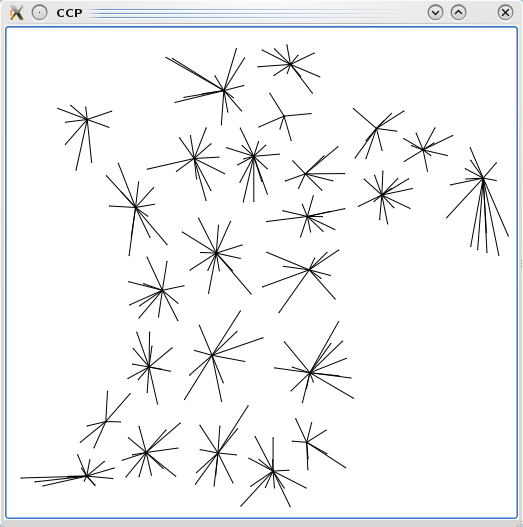
\includegraphics[scale=0.4,keepaspectratio=true]{../TCC-I/imagens/cluster_Density_SJC4a.png}\label{a}
 % cluster_Density_SJC4a.png: 523x527 pixel, 83dpi, 16.00x16.13 cm, bb=0 0 454 457
}
\subfloat[]{
 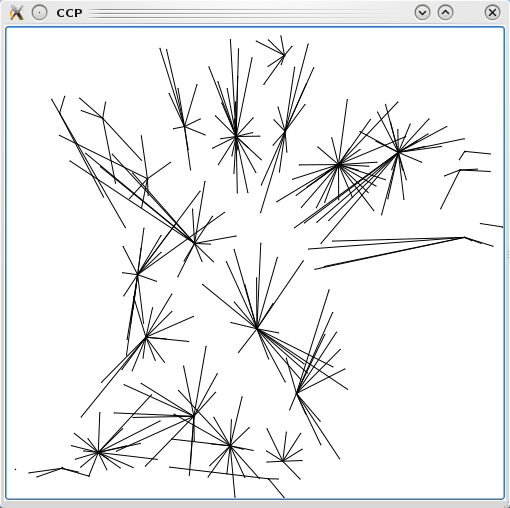
\includegraphics[scale=0.4,keepaspectratio=true]{../TCC-I/imagens/cluster_Farthest_SJC4a.png}\label{b}
 % cluster_Farthest_SJC4a.png: 510x508 pixel, 83dpi, 15.61x15.54 cm, bb=0 0 442 441
}\\
\subfloat[]{
 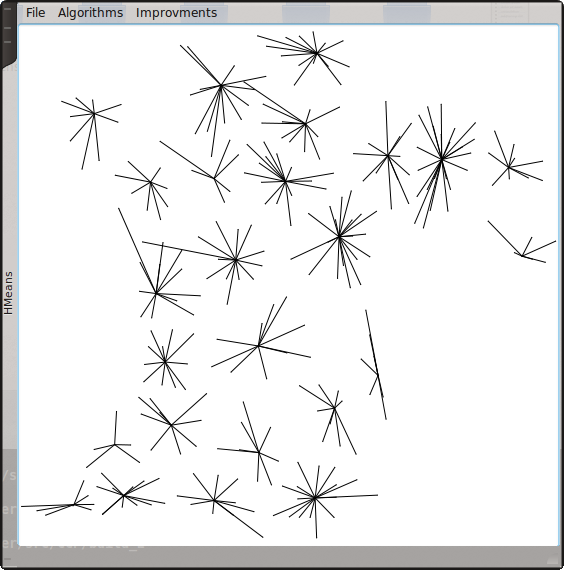
\includegraphics[scale=0.4, bb=0 0 423 427]{./images/HMeans_Example.png}\label{c}
 % HMeans_Example.png: 564x570 pixel, 96dpi, 14.92x15.08 cm, bb=0 0 423 427
}
\subfloat[]{
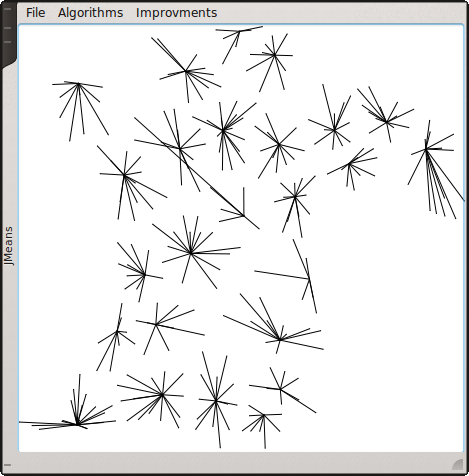
\includegraphics[scale=0.5, bb=0 0 423 427]{./images/JMeans_Example.png}\label{d}
}
\par

\caption[Compara��o algumas solu��es das heur�sticas]{\label{fig:CCP-compara=0000E7=0000E3o}A solu��o gerada pelas heur�stica
Density \subref{a}, Farthest \subref{b}, HMeans\subref{c} e JMeans\subref{d}. Para todas solu��es foi calculado com o mesmo valor de p (n�mero de agrupamentos).}
\end{centering}
\end{figure}

\subsection{Random Density}
\sloppy A heur�stica proposta por \cite{ahmadi2004density} produz solu��es muito boas, mas na grande maioria das vezes cai em um m�nimo local, tanto que o refinamento da solu��o obtida apresentado no mesmo artigo � atrav�s da altera��o dos dados de entrada, pela perturba��o de alguns indiv�duos e recalculando os novos agrupamentos. Com esses novos agrupamentos � recalculado a fun��e objetivo levando em considera��o o posicionamento original dos indiv�duos. A ideia de densidade utilizada por Ahmadi d� uma boa ideia da prov�vel localiza��o dos indiv�duos candidatos a centros de agrupamentos. Usando dessa ideia e da t�cnica construtiva/desconstrutiva tamb�m representado no mesmo trabalho, criamos o algoritmo \ref{alg:RandomDensity}:

\begin{algorithm}[hpt]
\caption{{RandomDensity}\label{alg:RandomDensity}}
\begin{algorithmic}[1]

\STATE $X \leftarrow I$
\STATE $Y \leftarrow \emptyset$ \COMMENT {conjunto de pontos j� atribu�dos}
\STATE $k=0;$
\WHILE {$k < p$}
  \STATE $k\leftarrow k+1$
  \FORALL {$i \in X$}
    \STATE $V \leftarrow EncontraVizinhos (i)$
    \STATE CalculaDensidade(i, V)
  \ENDFOR
  \STATE $newC \leftarrow GetRandonDensity(X)$ \COMMENT {Seleciona um dos $p$ pontos com maior densidade.}
  \STATE $C_{k} \leftarrow newC$
  \STATE $Y \leftarrow Y\cup EncontraVizinhos (newC)$
  \STATE $X \leftarrow X\setminus Y$
  \IF {$k \geq 2$}
    \STATE $EncontreOsMelhoresAgrupamentos(C,Y)$
  \ENDIF
\ENDWHILE
\STATE $EncontreOsMelhoresAgrupamentos(C,I)$
\end{algorithmic}

\end{algorithm}

Note que agora na linha 10 do algoritmo \ref{alg:RandomDensity} n�o � mais selecionado o indiv�duo com maior densidade, mas sim um dos pontos com maior densidade, retirando o movimento guloso do algoritmo original que acabava por conduzir sempre a uma mesma solu��o. Com essa pequena altera��o consegu�mos solu��es muito boas e tamb�m que permitem uma aplica��o de busca local para melhorar o resultado obtido. Conseguimos, com essa pequena altera��o, obter solu��es m�dias melhores que os demais m�todos na maioria das inst�ncias. Em contrapartida, o tempo de processamento computacional aumentou. Isso se deve pela necessidade de maior n�mero de itera��es no procedimento $EncontreOsMelhoresAgrupamentos(C,Y)$ (\ref{alg:;EncontreOsMelhoresAgrupamentos}), agora que as escolhas de indiv�duos como centros pode gerar uma maior necessidade de movimenta��o dos indiv�duos entre os agrupamentos na fase de constru��o/desconstru��o.

Uma forma de obter solu��es boas � ap�s gera-las com alguma heur�stica, aplicar algum m�todo de busca local, procurando na solu��o obtida uma solu��o melhor na vizinhan�a da solu��o atual.

\section{Busca Local}
Usando os movimentos descritos por \cite{osman1994capacitated} de interchange (interc�mbio) e shift (mudan�a) temos os mecanismos de gera��o de solu��es vizinhas � solu��o atual. Ambos movimentos respeitam a capacidade de cada agrupamento, n�o inserindo um indiv�duo em um agrupamento que ultrapasse sua capacidade.

O movimento shift � uma troca simples onde apenas � removido um indiv�duo $i$ de um agrupamento $C$ e o mesmo indiv�duo � inserido em um outro agrupamento $C'$, sendo $C \neq C'$ e $C'$ possui capacidade suficiente para atender a demanda de $i$. Esse movimento n�o permite grande explora��o da vizinhan�a, uma vez que para execut�-lo � necess�rio que exista uma capacidade ociosa nos agrupamentos para receber novos pontos. Na figura \ref{shiftExample} � apresentado um exemplo de movimento shift executado em uma solu��o v�lida do problema.

\begin{figure}[ht]
\begin{centering}
\subfloat[]{
 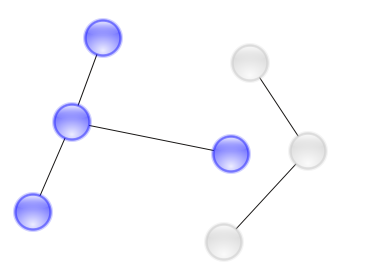
\includegraphics[scale=0.6]{../apresentacao_andamento/before_shift.png}% \label{a}
 % before_shift.png: 414x232 pixel, 96dpi, 10.95x6.14 cm, bb=0 0 310 174

}
\subfloat[]{
 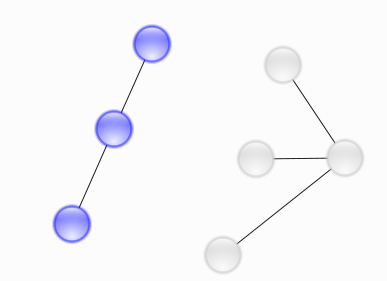
\includegraphics[scale=0.6]{../apresentacao_andamento/after_shift.png}% \label{b}
 % after_shift.png: 414x232 pixel, 96dpi, 10.95x6.14 cm, bb=0 0 310 174
}
\par
\caption[Exemplo movimento Shift]{Em \ref{a} temos uma solu��o com 2 agrupamentos e em \ref{b} uma solu��o vizinha ap�s movimento de shift.}\label{shiftExample}
\end{centering}
\end{figure}


O movimento de interchange, visa trocar um indiv�duo $i'$ de um agrupamento $C'$ por um outro indiv�duo $i$ de um outro agrupamento $C$, sendo $i \neq i'$ e $C \neq C'$.
Esse movimento permite que sejam encontradas novas solu��es vizinhas a atual mesmo quando os agrupamentos se encontram com demanda alta (pouca capacidade dispon�vel), pois a troca � feita em um �nico momento sem que necessariamente um agrupamento deva ter capacidade suficiente para receber um ponto extra. Nas figuras em \ref{interchangeExample}, pode ser visto o movimento interchange, sendo em (a) os agrupamentos existentes e que permitem a troca dos pontos entre si pelo movimento interchange e em (b) a solu��o obtida pelo movimento.
\begin{figure}[ht]
\begin{centering}
\subfloat[]{
 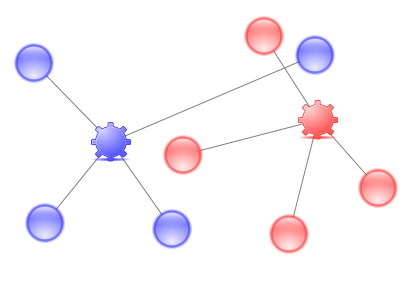
\includegraphics[scale=0.6]{../apresentacao_andamento/before_interchange.png}% \label{a}
 % before_shift.png: 414x232 pixel, 96dpi, 10.95x6.14 cm, bb=0 0 310 174
}
\subfloat[]{
 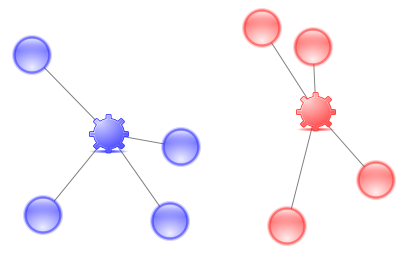
\includegraphics[scale=0.6]{../apresentacao_andamento/after_interchange.png}% \label{b}
 % after_shift.png: 414x232 pixel, 96dpi, 10.95x6.14 cm, bb=0 0 310 174
}
\par
\caption[Exemplo movimento interchange]{Em \ref{a} temos uma solu��o com 2 agrupamentos e em \ref{b} uma solu��o vizinha ap�s movimento de interchange.} \label{interchangeExample}
\end{centering}
\end{figure}

Ao final de cada movimento, as medianas s�o recalculadas de modo a minimizar a fun��o objetivo do problema.


Para busca local, foram implementados 2 algoritmos, ambos usando uma busca gulosa na vizinhan�a por solu��es com valores da fun��o objetivo menores e cada um deles usando um dos movimentos acima descritos.

Para o algoritmo com o movimento shift, chamado internamente na ferramenta computacional ShiftHillClimb, ele faz uma busca completa de todas possibilidades de mudan�a do indiv�duo do agrupamento atual para os demais, efetuando a troca do indiv�duo que d� um maior ganho para a fun��o objetivo. Ele segue o algoritmo apresentado em \ref{alg:ShiftHillClimb}. Esse algoritmo � executados iterativamente at� que n�o existam solu��es vizinha com uma fun��o objetivo menor (um m�nimo local) e tem  complexidade de $O(n\cdot p)$ para cada itera��o.
\begin{algorithm}
\caption{{ShiftHillClimb}\label{alg:ShiftHillClimb}}
\begin{algorithmic}[1]
\STATE $MelhorSol \leftarrow AtualSol $
\REPEAT
\STATE $NovaSol \leftarrow MelhorSol$
\FORALL {$i \in I$}
\STATE Procura a melhor troca de i para um dos demais p-1 agrupamentos
\ENDFOR
\STATE $NovaSol \leftarrow melhor movimento de Shift$
\UNTIL{NovaSol $<$ MelhorSol }
\end{algorithmic}
\end{algorithm}

O algoritmo de busca local implementado usando o movimento de interchange, originalmente tentava executar a troca de um ponto com todos os pontos dos demais agrupamentos que n�o o seu. Isso o deixava com uma complexidade $O(n \cdot (p-1) \cdot \frac{n}{p})$, algo muito pr�ximo a $O(n^{2})$ para cada itera��o.Para reduzir o espa�o de busca do algoritmo, uma vez que muitos dos interc�mbios n�o geram solu��es melhores, implementamos o algoritmo \ref{alg:InterchangeHillClimb}.
\begin{algorithm}
\caption{{InterchangeHillClimb}\label{alg:InterchangeHillClimb}}
\begin{algorithmic}[1]
\STATE $MelhorSol \leftarrow AtualSol $
\STATE $Q \leftarrow \lceil p * 0.3 \rceil$
\STATE $K \leftarrow \lfloor \frac{n}{p}\cdot 0.5 \rfloor$
\REPEAT
\STATE $NovaSol \leftarrow MelhorSol$
\FORALL {$ i \in I $ }
\FORALL {$ j \in K \text{ agrupamentos mais pr�ximos de } i $}
\STATE $Procura de i com Q \text{indiv\'{i}duos} \in j mais \text{pr�ximos}$
\ENDFOR
\ENDFOR
\STATE $NovaSol \leftarrow melhor movimento de interchange$
\UNTIL{NovaSol $<$ MelhorSol }
\end{algorithmic}
\end{algorithm}

\sloppy Com essa metodologia, conseguimos reduzir o espa�o de busca pela elimina��o das solu��es que n�o apresentariam redu��es no valor da fun��o objetivo. Uma r�pida analise na complexidade $O(n \cdot Q \cdot K)$, onde Q = 30\% dos agrupamentos ($p\cdot 0.3$) e K � 50\% da m�dia de pontos por agrupamento ficando uma complexidade muito pr�xima de $O(n)$ para cada itera��o.

O n�mero de itera��es para cada um desses algoritmos � inversamente proporcional a qualidade da solu��o, uma vez que uma solu��o boa tem poucas, ou at� mesmo nenhuma, solu��es com valor da fun��o objetivo melhor que a sua, o que demanda menos passos no algoritmo para chegar em m�nimo loca.
\chapter{Ferramenta Computacional}
Para melhor executar os estudos do problema, foi desenvolvida uma ferramenta computacional que prove a visualiza��o dos resultados, permite programar execu��es de algoritmos para arquivos abertos, oferecendo com a op��o de aplicar ou n�o os algoritmos de busca local na solu��o final, al�m de permitir rodar arquivos em lote.
Os resultados s�o aprentado em uma saida de texto e salvos em um arquivo o que permite manter um hist�rico das execu��es para cada arquivo.

\begin{figure}[ht]
 \centering
 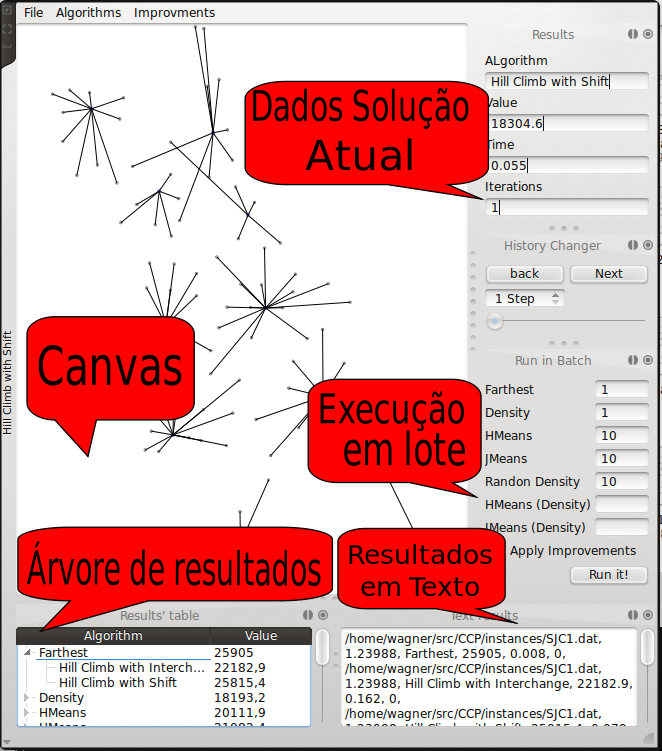
\includegraphics[viewport=0 0 496 563, scale=0.5]{./images/CCPFerramentaNumerada.png}
 % CCPFerramentaNumerada.png: 662x751 pixel, 96dpi, 17.51x19.87 cm, bb=0 0 496 563
 \caption{Tela principal da ferramenta desenvolvida\label{fig:FerramentaNossa}}
\end{figure}

Os processamentos de algoritmos contrutivo e de busca local solicitados pelo utilizador, s�o armazenados em um fila sendo que o processamento deles ocorre em uma thread separada, permitindo a interface do utilizador n�o fique bloqueada enquanto o dados s�o processados.

Como os algoritmos de busca local podem ser aplicados nas solu��es geradas por eles, foi implementada uma organiza��o dos resultados derivados em formato de �rvore. Essa �rvore permite a navega��o nela, mostrando na janela de visualiza��o de resultados (canvas) os resultados nela selecionados.

Como alguns algoritmos tem a escolha das medianas iniciais de forma aleat�ria, � poss�vel indicar quantas vezes os algoritmos com essa propriedade sejam executados.

Para o desenvolvimento foi escolhida a linguagem de program��o C++ fazendo uso do paradigma orientado a objetos e utilizado como compilador o GCC\sigla{GCC}{Cole��o de Compiladores GNU - GNU Compiler Collection} da GNU\sigla{GNU}{GNU N�o � Unix - GNU is Not Unix}. A interface foi construida utilizando o framework Qt da Nokia, o qual serviu n�o apenas de base da interface, mas tamb�m para os casos de teste, comunica��o entre objetos, processamento de arquivos e concorr�ncia (threads). Para o gerenciamento de vers�es do projeto foi utilizado o git, tendo os c�digos disponibilizados no reposit�rio http://github.com/wiglot/CCP.

Para efetuar a gera��o dos arquivos makefiles, utilizados para executar a compila��o da ferramenta, foi utilizado o gerador de makefiles CMake pela facilidade de uso, poder no controle de decis�es e por possibilitar a execu��o dos casos de teste de forma automatizada pelo pacote CTest, o qual faz parte do pr�prio CMake.

Como contribui��o, tamb�m foi desenvolvido uma primeira vers�o de um plugin (biblioteca din�mica) para o Rocs \cite{Rocs2010} do KDE-EDU (conjunto de softwares educacionais do KDE), permitindo uma poss�vel intera��o com a solu��es geradas pelos algoritmos aqui trartados atrav�s de comandos na linguagem java script e tamb�m a cria��o de algoritmos para an�lise de tais solu��es. Essa primeira vers�o do plugin permite a abertura de arquivos do problema CCP e a execu��o de algum dos algoritmos desenvolvidos aqui. Na figura \ref{fig:DuasFerramentas} temos um exemplo das duas ferramentas com a mesma inst�ncia e o mesmo algoritmo rodado (density).

\begin{figure}[ht]
\begin{center}
\subfloat[]{
 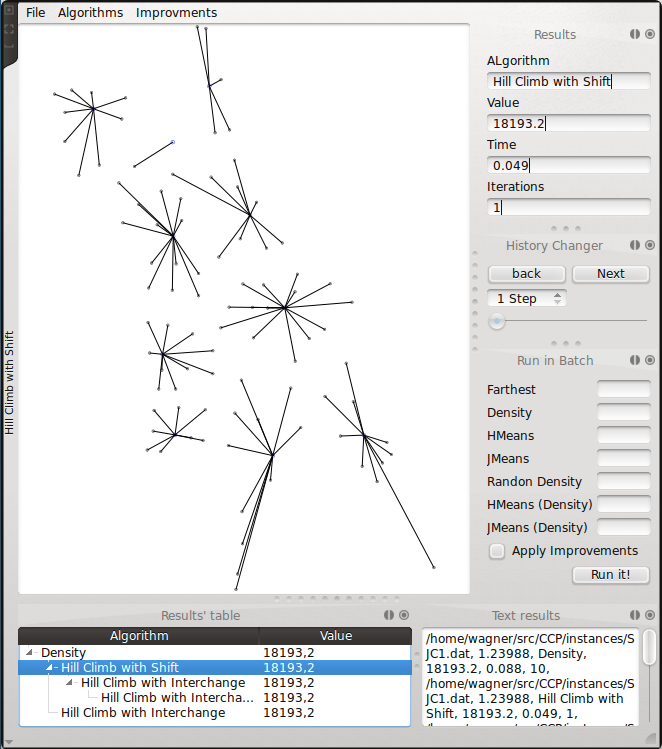
\includegraphics[scale=0.36]{./images/CCPFerramenta.png} \label{fig:ccpferramenta}
 % CCPFerramenta.png: 662x749 pixel, 96dpi, 17.51x19.81 cm, bb=0 0 496 562
}
\subfloat[]{
 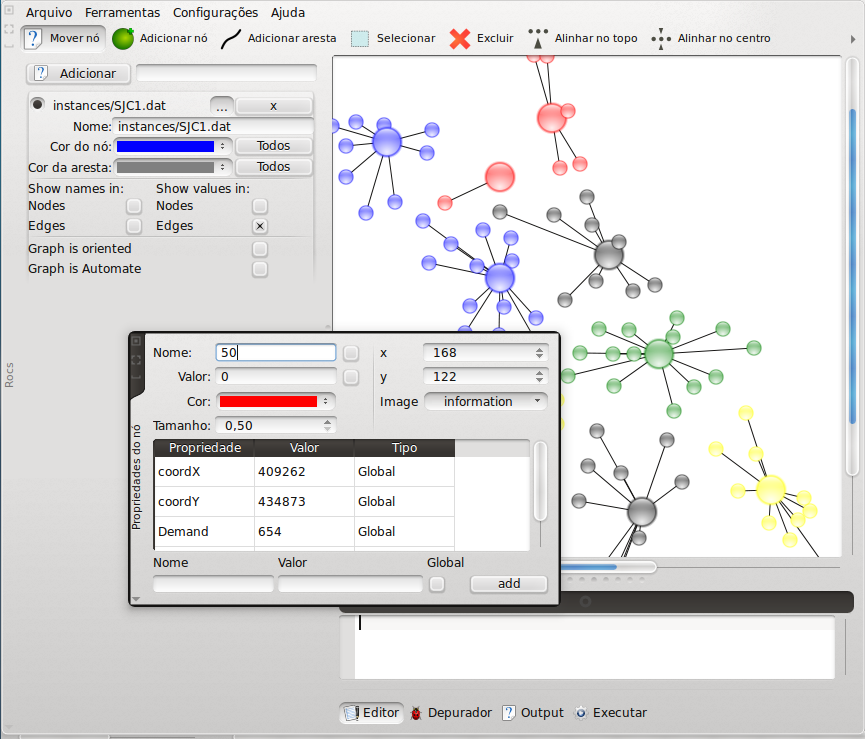
\includegraphics[scale=0.36]{./images/RocsCCP.png} \label{fig:rocsCCP}
 % RocsCCP.png: 865x739 pixel, 96dpi, 22.88x19.55 cm, bb=0 0 649 554
}
\par
\caption{Rocs e a ferramenta desenvolvida}{Duas ferramentas, a desenvolvida nesse trabalho \subref{fig:ccpferramenta} e o Rocs \subref{fig:rocsCCP} ambos com os mesmos algoritmos rodados sobre a mesma inst�ncia \label{fig:DuasFerramentas}}
\end{center}
\end{figure}

Tanto o plugin para o Rocs quanto a ferramenta desenvolvida como um todo, est�o licenciados pela GPL, o que permite a futuros estudantes e pesquisadores utilizarem e modificarem a ferramenta conforme suas necessidades, n�o necessitando recriar todo um sistema do zero.

Nos anexos est�o apresentados os diagramas UML da ferramenta. A ferramenta est� dividida nas seguintes bibliotecas:
\begin{description}
\item {CCPAlgorithms:} Algoritmos construtivos. N�o inclui busca local nem o controle da execu��o dos algoritmos (concorr�ncia)
\item {CCPClusterView:} Define as janelas e itens gr�ficos.
\item {CCPIOlib:} Tratam da entrada de dados dos arquivos.
\item {CCPModel:} Representa o problema com todas estruturas b�sicas para representar uma inst�ncia a solu��o. Cuida tamb�m do enfileiramento dos pedidos de execu��o dos algoritmos e buscas locais.
\end{description}

\chapter{Estudo das Caracter�sticas das Inst�ncias}
chamamos de folga a diferen�a entre a soma das demanda e a capacidade total oferecida. Para comparar entre as diferentes inst�ncias, utilizamos a formula \ref{folga}:
% \begin{equation}
\begin{align}
 F &= \frac{\sum_{p\in P} p_{cap} }{\sum_{i \in I} i_{dem}} \label{folga}
\end{align}

Onde $i_{dem}$ � a demanda do indiv�duo $i$ e $p_{cap}$ a capacidade do agrupamento $p$. $F$ � maior que 1 se a demanda total � menor que a capacidade total. Para valores de $F$ muito pr�ximos a 1, mas maiores que 1, as heur�sticas tendem a n�o conseguir nem mesmo uma solu��o fact�vel, principalmente heur�sticas que utilizam de procedimentos gulosos para aloca��o de indiv�duos, como por exemplo a escolha do agrupamento com mediana mais pr�xima do indiv�duo a ser alocado. Para valores menores que 1 n�o existe uma solu��o v�lida para a inst�ncia, uma vez que existe maior demanda que oferta (capacidade).

Para o caso de $ \sum_{i \in I} i_{dem} \geq p_{cap},\forall p \in P $ podemos dizer que o problema � equivalente ao problemas das P-medianas n�o capacitado, uma vez que a capacidade n�o chega a ser uma restri��o no problema e todos os indiv�duos podem ser associados a apenas uma agrupamento.

Essa ultima coloca��o mostra o quanto o valor de folga pode interferir na gera��o de solu��es das inst�ncias.
Nas inst�ncias in�ditas apresentadas aqui, modificamos a
%  F =
% \end{equation}


Mostrar do estudo da folga, diferen�a de demanda entre os pontos (min, m�x)

Apresentar tamb�m estudo de dispers�o dos pontos usando centro de massa com vari�ncia da capacidade dos pontos criados, e dist�ncia entre os pontos e o centro de massa (ser� que vai dar tempo??).


\chapter{Resultados Computacionais}
Apresenta��o e an�lise dos resultados obtidos

Na tabela \ref{tab:valoresInstancias} apresentamos os valores obtidos para os 5 algoritmos implementados. Para os algoritmos que utilizam de aleatoriedade na sele��o dos pontos, eles foram executados 10 vezes cada um e foi tirada a m�dia das 10 execu��es. Mais a frente mostraremos a vari�ncia dos resultados obtidos.
\begin{table}[htp]
\begin{center}
\caption {\\Valores da obtidos das inst�ncias pelos algoritmos construtivos.\label{tab:valoresInstancias}}
\begin{tabular}{lrrrrrrr}
\toprule
Inst�ncia &\multicolumn{1}{c}{n}&\multicolumn{1}{c}{p}& \multicolumn{1}{c}{Density}
          & \multicolumn{1}{c}{Farthest} & \multicolumn{1}{c}{H-Means}
          & \multicolumn{1}{c}{J-Means}  & \multicolumn{1}{c}{Random Density} \\
\midrule
%%%%%%%Valores
SJC1  &  100&  10&18.193,2 & 25.905,0 &19.169,4 &20.247,9 &17.693,9 \\
SJC2  &  200&  15& 34.520,4  &52.121,3 &35.179,5 &34.591,2&34.147,2 \\
SJC3a &  300&  25& 47.976,7  &76.345,3 &49.231,8 &48.140,4  &45.907,9 \\
SJC3b &  300&  30& 42.501,7  &69.956,2 & 42.607,4 &42.329,0  &42.151,3 \\
SJC4a &  402&  30& 65.655,4 &103.171,0 &66.763,9  &67.595,4 &63.602,9 \\
SJC4b &  402&  40& 54.077,1  &92.948,9 & 57.092,1 &55.412,2 &54.438,2 \\
SJC5  &  402&  20& 97.681,6  &134.798,0 & 99.502,9  &100.117,0  &86.325,5 \\
AESM\_10 &  1142& 21& 96.738,2 & 20.519,8     &  15.482,0 & 16.409,9 &  15.251,7 \\
AESM\_20 &  & & 97.798,8 & 16.466,2  &  16.472,7 & 13.753,0   &  11.665,8 \\
AESM\_30 &  & & 69.541,8 & 16.582,9   &  13.504,5 &  12.859,9&  11.626,2\\
AECP\_10 &  324&  10& 27.877,4 &   6.447,6 &  6.482,0& 6.846,3   &   6.458,0 \\
AECP\_20 &  & & 9.889,6  & 6.173,6   &   5.900,1 & 6.331,2   &   5.835,2  \\
AECP\_30 &  & & 8.374,6  &6.155,2    &5.646,0 & 5.608,7 &      5.799,3 \\
AENH\_10 &  2327& 17& 86.174,4 & 24.735,9 & 26.241,5& 26.056,1 &  23.910,3 \\
AENH\_20 &  && 73.593,2   & 24.549,9 &  24.860,3   & 24.218,4  &   22.826,4 \\
AENH\_30 &  && 74.153,2&25.785,4 & 24.913,3 & 27.481,7 & 23.977,9 \\
AELJ\_10 &  646& 14& 32.398,0 & 9.174,7   &9.982,1 & 9.703,8&10.177,6 \\
AELJ\_20 &  & & 32.248,7 & 8.798,5    &8.109,5 & 8.283,7& 8.472,1 \\
AELJ\_30 &  & & 27.915,8 &8.735,7   &7.535,1  &7.645,9 & 8.086,4 \\
AEAL\_10 &  448&15& 29.700,4 & 10.850,5  &10.933,5& 11.216,0 &10.838,4 \\
AEAL\_20 &  && 27.219,8 &10.763,5   &9.164,8 & 9.336,6 & 9.026,3 \\
AEAL\_30 &  && 26.814,7 & 10.752,1  &8.837,1 & 9.026,4 & 8.818,8\\
\bottomrule
\end{tabular}
\end{center}
\end{table}

As solu��es com aleatoriedade tem os desvios padr�o apresentados na tabela \ref{tab:stdDev}.

\begin{threeparttable}[htp]
\begin{center}
\caption {\\Desvio padr�o dos valores obtidos pelos algoritmos com aleatoriedade.\label{tab:stdDev}}
\begin{tabular}{lrrrrrr}
\toprule
Inst�ncia & \multicolumn{2}{c}{H-Means}
          & \multicolumn{2}{c}{J-Means}  & \multicolumn{2}{c}{Random Density} \\

 & \multicolumn{1}{c}{M�dia}& \multicolumn{1}{c}{DP\tnote{1}}
 & \multicolumn{1}{c}{M�dia}& \multicolumn{1}{c}{DP}
 & \multicolumn{1}{c}{M�dia}& \multicolumn{1}{c}{DP} \\
\midrule
%%%%%%%Valores
SJC1     &20.066,6 &619,3  &21.214,0   &966,1  &18.430,9   &653,4  \\
SJC2     &36.767,7  &1.205,0    &36.109,6   &1.269,5    &34.700,3   &355,3  \\
SJC3a    &50.651,7  &1.019,7    &50.041,5   &1.631,5    &47.394,5   &954,9  \\
SJC3b    &45.381,0  &1.433,6    &44.164,0   &1.257,6    &42.872,4   &333,9 \\
SJC4a    &73.892,6  &7.058,7    &69.357,4   &884,2  &65.340,5   &1.219,2  \\
SJC4b    &62.457,6  &5.679,8    &56.585,4   &640,5  &55.867,4   &715,6\\
SJC5     &102.325,8    &1.894,5    &109.244,7  &9.669,6    &91.377,1   &2.616,6  \\
AESM\_10    &22.434,58 &5.723,65   &21.166,50  &3.880,00   &19.874,29  &2.410,11 \\
AESM\_20    &19.000,31  &2.825,51   &16.322,42  &1.568,66   &14.684,51  &1.445,29\\
AESM\_30    &16.080,65  &1.764,01   &15.418,38  &1.564,28   &13.392,51  &928,93\\
AECP\_10    &6.594,54   &61,89      &8.130,36   &3.288,99   &6.560,09   &112,85 \\
AECP\_20    &6.318,05   &349,87     &6.702,14   &564,02 &6.107,97   &144,67\\
AECP\_30    &10.319,98  &4.241,99   &7.239,48   &2.448,47   &6.482,20   &1.455,36\\
AENH\_10    &28.441,94  &2.038,19   &29.939,45  &7.388,23   &24.126,65  &503,47\\
AENH\_20    &26.918,98  &1.808,29   &26.577,87  &1.844,80   &23.861,87  &742,50\\
AENH\_30    &25.554,47  &693,58     &28.506,26  &7.758,78   &23.412,79  &561,11\\
AELJ\_10    &14.735,16  &4.248,58   &11.158,81  &1.699,12   &10.782,29  &372,57\\
AELJ\_20    &14.386,39 &5.332,40    &8.883,50   &528,24 &8.543,30   &244,10\\
AELJ\_30    &14.186,13   &5.082,51   &8.491,72   &601,71 &8.138,73   &70,00 \\
AEAL\_10    &12.527,41   &4.291,75   &11.779,82  &330,40 &10.901,17  &68,26 \\
AEAL\_20    &12.438,82  &4.874,71   &10.504,24  &792,56 &9.812,93   &732,16 \\
AEAL\_30    &11.998,70  &3.951,95   &10.980,83  &2.566,85   &9.297,77   &648,16 \\
\bottomrule
\end{tabular}
\begin{tablenotes}
 \item[1]Desvio Padr�o
\end{tablenotes}
\end{center}
\end{threeparttable}


Os tempos computacionais tomados por cada algoritmo para gerar as solu��es apresentadas anteriormente, � apresentado na tabela
\ref{tab:TemposInstancias}.

\begin{table}[htp]
\begin{center}
\caption {\\Tempo (em segundos) para c�lculo das solu��es.\label{tab:TemposInstancias}}
\begin{tabular}{lrrrrrrrrrrrr}
\toprule
Inst�ncia & \multicolumn{1}{c}{Farthest} & \multicolumn{1}{c}{Density} & \multicolumn{1}{c}{H-Means}
          & \multicolumn{1}{c}{J-Means}  & \multicolumn{1}{c}{Random Density} \\
\midrule
%%%%%%%Valores
SJC1  &  0,009  &0,085   &0,002  & 0,177  & 0,092\\
SJC2  &  0,030  &0,393   &0,003  & 3,002  & 0,726\\
SJC3a &  0,036  &1,678   &0,013  &28,983  & 3,568 \\
SJC3b &  0,046  &1,839   &0,010  &50,773  & 3,484 \\
SJC4a &  0,056  &6,396   &0,021  &74,550  &20,727 \\
SJC4b &  0,054  &6,254   &2,981  &199,509 &8,679\\
SJC5  &  0,050  &5,110   &0,026  &49,322  &6,070 \\
AESM\_10 &   0,87   & 108,90  &0,19 &482,74  &  358,33 \\
AESM\_20 &   0,08   & 53,41  &0,16& 530,03 &266,70 \\
AESM\_30 &   0,08   &57,73   &0,15&375,48  &141,06\\
AECP\_10 &   0,07   & 2,06   & 0,02 & 3,04  & 2,36 \\
AECP\_20 &   0,01   & 1,79   & 0,01 & 2,53  & 3,08 \\
AECP\_30 &   0,01   & 1,39   & 0,01 & 0,86 & 2,24 \\
AENH\_10 &   4,14   &458,44   &1,21 &  4.857,36  &  1.407,63\\
AENH\_20 &    0,26  & 461,44  &1,34 &  3.838,05  & 1.572,15\\
AENH\_30 &   0,26   & 361,01  &0,76 &  3.281,53  &  961,22\\
AELJ\_10 &   0,04   & 7,96   & 5,81 & 54,66 & 55,24 \\
AELJ\_20 &   0,03   & 10,57  & 6,18 & 82,39 & 25,52\\
AELJ\_30 &   0,04   & 1,39   &0,04  &53,57  &20,55  \\
AEAL\_10 &  0,18    & 13,04  &0,03  &10,59  &13,66 \\
AEAL\_20 &  0,02    & 6,21   &0,03  &24,00  &9,03 \\
AEAL\_30 &  0,03    &4,40    &0,03  &19,47  &15,70\\
\bottomrule
\end{tabular}
\end{center}
\end{table}


% \begin{table}[htp]
% \begin{center}
% \caption {\\Valores da obtidos das inst�ncias pelos algoritmos construtivos.\label{tab:valoresInstancias}}
% \begin{tabular}{lrrrrrrrrrr}
% \toprule
% Inst�ncia & \multicolumn{2}{c}{Density} & \multicolumn{2}{c}{Farthest} & \multicolumn{2}{c}{H-Means}
%           & \multicolumn{2}{c}{J-Means}  & \multicolumn{2}{c}{Random Density} \\
% &\multicolumn{1}{c}{Valor}&\multicolumn{1}{c}{T(s)}
% &\multicolumn{1}{c}{Valor}&\multicolumn{1}{c}{T(s)}
% &\multicolumn{1}{c}{Valor}&\multicolumn{1}{c}{T(s)}
% &\multicolumn{1}{c}{Valor}&\multicolumn{1}{c}{T(s)}
% &\multicolumn{1}{c}{Valor}&\multicolumn{1}{c}{T(s)} \\
% \midrule
% %%%%%%%Valores
% SJC1  &18.193,2 &0,085& 25.905,0 & 0,009 &19.169,4 &0,002&20.247,9 &0,177 &99999 &0,1\\
% SJC2  & 34.520,4  &0,393&52.121,3 &0,030&35.179,5&0,003&34.591,2&3,002&99999 &0,1\\
% SJC3a & 47.976,7  &1,678&76.345,3&0,036&49.231,8&0,013&48.140,4& 28,983 &99999 &0,1\\
% SJC3b & 42.501,7  &1,839&69.956,2& 0,050& 42.607,4&0,010&42.329,0&50,773 &99999 &0,1\\
% SJC4a & 65.655,4  &6,396&103.171,0 &0,056&66.763,9&0,021&67.595,4&74,550 &99999 &0,1\\
% SJC4b & 54.077,1  &6,254&92.948,9 &0,054& 57.092,1&2,981&55.412,2&199,51 &99999 &0,1\\
% SJC5 & 97.681,6  &5,110&134.798,0 &0,050& 99.502,9 &0,026&100.117,0&49,322 &99999 &0,1\\
% AESM\_10 & 99999 &0,1&99999 &0,1&99999 &0,1&99999 &0,1 &99999 &0,1\\
% AECS\_10 & 99999 &0,1&99999 &0,1&99999 &0,1&99999 &0,1 &99999 &0,1\\
% AENH\_10 & 99999 &0,1&99999 &0,1&99999 &0,1&99999 &0,1 &99999 &0,1\\
% AESL\_10 & 99999 &0,1&99999 &0,1&99999 &0,1&99999 &0,1 &99999 &0,1\\
% AESM\_20 & 99999 &0,1&99999 &0,1&99999 &0,1&99999 &0,1 &99999 &0,1\\
% AECS\_20 & 99999 &0,1&99999 &0,1&99999 &0,1&99999 &0,1 &99999 &0,1\\
% AENH\_20 & 99999 &0,1&99999 &0,1&99999 &0,1&99999 &0,1 &99999 &0,1\\
% AESL\_20 & 99999 &0,1&99999 &0,1&99999 &0,1&99999 &0,1 &99999 &0,1\\
% AESM\_30 & 99999 &0,1&99999 &0,1&99999 &0,1&99999 &0,1 &99999 &0,1\\
% AECS\_30 & 99999 &0,1&99999 &0,1&99999 &0,1&99999 &0,1 &99999 &0,1\\
% AENH\_30 & 99999 &0,1&99999 &0,1&99999 &0,1&99999 &0,1 &99999 &0,1\\
% AESL\_30 & 99999 &0,1&99999 &0,1&99999 &0,1&99999 &0,1 &99999 &0,1\\
% \bottomrule
% \end{tabular}
% \end{center}
% \end{table}
Tomando como base os resultados apresentados por Lorena e por negreiros para as inst�ncias SJC, escolhemos os melhores resultados, que foram os apresentados por Lorena (CITE LORENA), apresentamos a tabela \ref{tab:CompResultados} onde temos os melhores resultado obtidos pelos trabalhos e por os implementados por n�s. Como pode ser visto, Lorena possui os melhores resultados, por isso servir�o de base para calcular a porcentagem que as demais solu��es se encontram acima de suas solu��es.


\begin{threeparttable}[ht]
\begin{center}
\caption {\\Compara��o dos resultados com a literatura.\label{tab:CompResultados}}
\begin{tabular}{lrrrrrrrrrrr} \hline

 &  \multicolumn{2}{c}{N\tnote{1}} &   \multicolumn{2}{c}{L\tnote{2}}   &  \multicolumn{2}{c}{TCC\tnote{3}}  &   \multicolumn{2}{c}{N(\%)}     &   \multicolumn{2}{c}{TCC(\%)}\\
   & \multicolumn{1}{c}{V\tnote{a}} &  \multicolumn{1}{c}{T\tnote{b}}& \multicolumn{1}{c}{V} &  \multicolumn{1}{c}{T}& \multicolumn{1}{c}{V} &  \multicolumn{1}{c}{T}& \multicolumn{1}{c}{V(\%)} &  \multicolumn{1}{c}{T(\%)}& \multicolumn{1}{c}{V(\%)} &  \multicolumn{1}{c}{T(\%)} \\ \hline
SJC1    &17288,9  &  0,02   & 17252,1  &   68,62  & 17693,9   &0,09   & 0,21 &  0,029 & 2,56  & 0,13 \\
SJC2    &33370,2 &   0,02   & 33223,6   &  2083,92 & 34147,2  &0,72   & 0,44 &  0,001 & 2,78  & 0,03 \\
SJC3a   &45335,1  &  0,08  & 45313,4   &  2604,92 & 45907,9  & 3,56  &  0,05 &  0,003 & 1,31 &  0,13 \\
SJC3b   &0        &        0 &  40634,9  &  867,68 & 42151,3  &3,48   &    |  &         |&  3,73 &  0,40 \\
SJC4a   &62026,9  &  0,08  & 61842,4   &   27717,11&  63602,9 &20,72 & 0,30 &  0,000 & 2,85 &  0,07 \\
SJC4b   &0         &       0 &  52396,5   &  4649,47 &54077,1  &6,25   &       |&        |&  3,21  & 0,13 \\
 \hline
\end{tabular}
\begin{tablenotes}
 \item[1]Negreiros \cite{negreiros2006capacitated}
 \item[2]Lorena \cite{negreiros2006capacitated}
 \item[3]Algoritmos implementados
\end{tablenotes}
\begin{tablenotes}[para]
 \item[]
 \item[a]Valor da fun��o objetivo,
 \item[b]Tempo gasto pelo algoritmo em segundos.
\end{tablenotes}
\end{center}

\end{threeparttable}



% Conclus�o - Obrg
\chapter*{Considera��es Finais}

% Neste trabalho apresentamos a aplica��o de heur�sticas e m�todos de otimiza��o para o problema de agrupamento capacitado. O problema de agrupamento capacitado � um problema que representa em parte o problema de despacho de ordens de servi�o, por isso ele foi estudado nesse trabalho, sendo o PDOS o nosso cen�rio de aplica��o. 

Apresentamos aqui neste trabalho uma vis�o do PDOS como um CCP, fazendo uso de m�todos j� existentes em um problema relativamente novo. Dos m�todos tratados, procuramos abordar os m�todos heur�sticos mais tratados da literatura e compara-los quando aplicados aos dados do PDOS.

Dentre os m�todos trabalhados, os que apresentaram melhores solu��es foram o Random density e o Density, sendo o primeiro uma varia��o do segundo, com a diferen�a de inserir elementos de aleatoriedade para escolha dos centros, n�o desconsiderando o c�lculo de densidade o qual nos d� um bom indicativo de onde devem ser inseridos os centros. Mas, apesar de os valores obtidos serem menores que os demais m�todos, o seu tempo de computa��o � cerca de 3 vezes mais alto que o levado pelo m�todo density, que para inst�ncias com grande n�mero de indiv�duos e de centros (por exemplo algumas inst�ncias com mais de 3.000 pontos e 600 agrupamentos), tem um tempo de computa��o bastante alto. Esse tempo elevado n�o desqualifica o uso do m�todo para essa classe de problemas, visto que os atendimentos s�o processados por cidades como apresentado nas inst�ncias AE e possuem grande n�mero de atendimentos e poucas equipes.

Dos demais m�todos, Farthest � uma heur�stica construtiva que gera solu��es de baixa qualidade mas rapidamente. HMeans gera solu��es de qualidade boas de modo at� mais r�pida que o �ltimo. JMeans gera solu��es de qualidade boa tamb�m, mas com a desvantagem de ser extremamente lento na fase de busca de novos centros e reassocia��o dos indiv�duos. Essa etapa dessa heur�stica pode sofrer melhorias para acelerar como um todo o algoritmo, visto que essa � a etapa mais repetida durante as itera��es. Como exemplo de melhoria seria a diminui��o do n�mero de centros removidos para a inser��o de um novo centro para apenas os centros mais pr�ximos a esse novo centro, evitando que se insira um centro onde j� exista um grande n�mero de centros.

As ferramentas computacionais tamb�m ficam como contribui��o para futuros trabalhos ou de base para implementa��o de novos algoritmos fornecendo toda representa��o do problema bem como a visualiza��o do mesmo para an�lise dos dados.

Para trabalhos futuros consideramos a utiliza��o de m�todos h�bridos, onde m�todos exatos seriam utilizados apenas para resolver subproblemas de complexidade menor e utiliza��o de buscas locais com espa�o de busca ampliado pela relaxa��o de algumas restri��es, gerando solu��es infact�veis mas com valor da fun��o objetivo melhor que serviria de base para uma nova busca por solu��es fact�veis em uma vizinhan�a que anteriormente n�o era alcan��vel ou que exigia grande refinamento na etapa de busca local. Outra considera��o a ser levada para os trabalhos futuros � que para aplica��es em cen�rios reais, deve-se levar em considera��o o deslocamento entre ordens de servi�o, o que iria contribuir para o aumento do tempo (valor da demanda) para a equipe que est� atendendo as ordens de servi�o e  a carga hor�ria das equipes poder ser vari�vel de uma para outra. Nesse caso ter�amos um problema heterog�neo quanto a capacidade e tamb�m ter�amos o problema de roteiriza��o das OS, sendo que ao calcular uma rota pode acontecer de aumentar tempo, devido a um maior deslocamento entre os novos atendimentos, para um valor al�m da capacidade da equipe, gerando uma solu��o infact�vel.

A parte construtiva das heur�sticas tamb�m permitem trabalhos futuros no que diz respeito a escolha de indiv�duos como centros iniciais. A escolha com o c�lculo por densidade se mostrou muito boa, mas se forem utilizados dados estat�sticos � poss�vel de se definir os centros com melhores caracter�scas. Para isso seria necess�rio a aplica��o de algum m�todo como o GRASP \cite{feo1989probabilistic} onde uma solu��o fornece dados para a gera��o de uma nova solu��o.
 %Inclui arquivo conclusao.tex

% ELEMENTOS P�S-TEXTUAIS
% Refer�ncias - Obrg
\bibliography{../bibitex/bibliography_CCP} %Seu arquivo Bibitex

% Gloss�rio
% Ap�ndice(s)

% Anexo(s)
% \appendix

% \part*{Anexos}


% \chapter*{Anexo A: Diagramas UML}
% \renewcommand{\thefigure}{A.\arabic{figure}}
%
% \begin{figure}[ht]
%  \centering
%  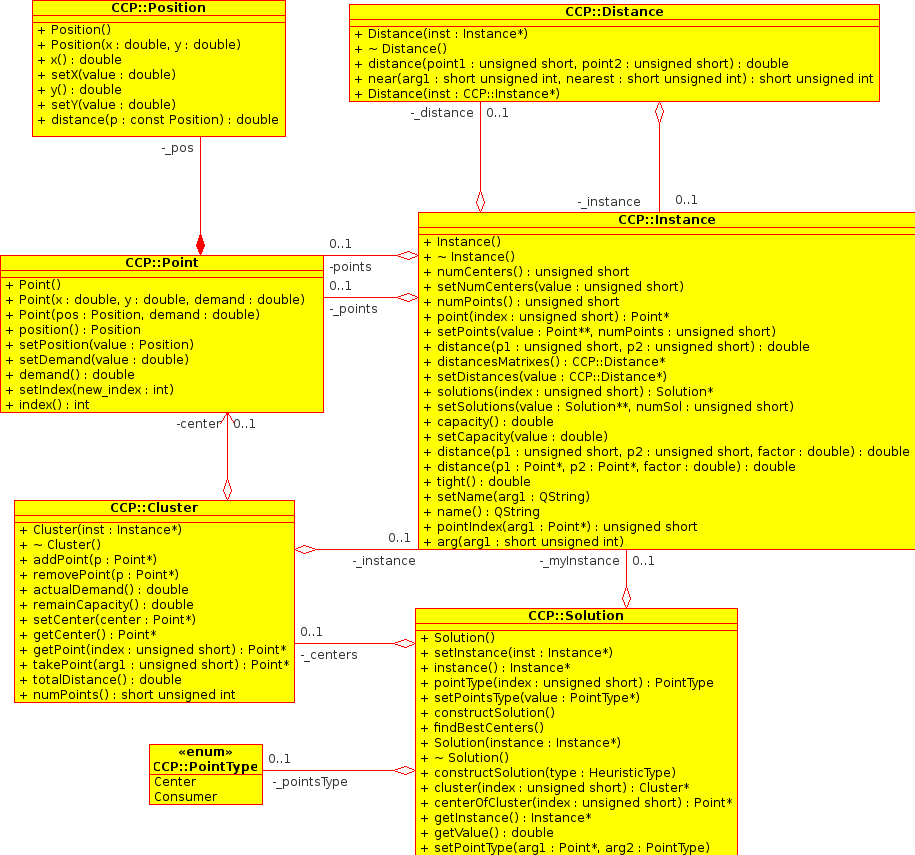
\includegraphics[bb=0 0 794 742,scale=0.4]{../TCC-I/imagens/Instance.png}
%  % Instance.png: 915x855 pixel, 83dpi, 28.00x26.16 cm, bb=0 0 794 742
% \caption{Classes que representam uma Inst�ncia e as solu��es }
% \end{figure}
%
% %
% % \begin{figure}
% %  \begin{center}
% %  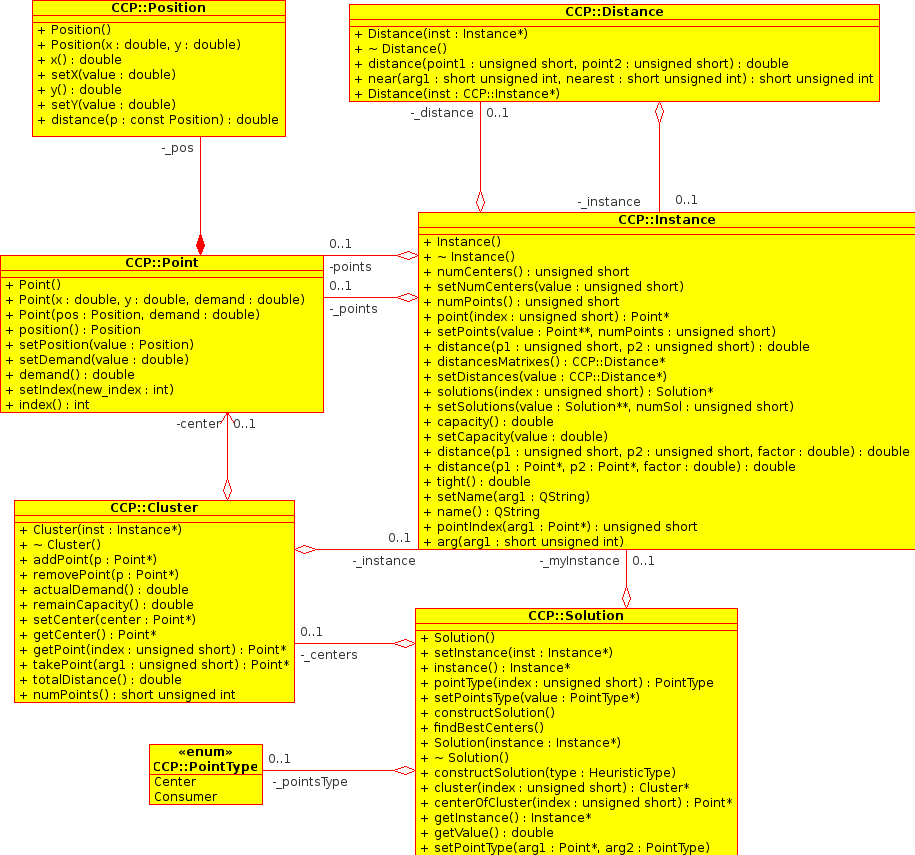
\includegraphics[scale=0.4]{../TCC-I/imagens/Instance.png}
% %  % Instance.png: 915x855 pixel, 83dpi, 28.00x26.16 cm, bb=0 0 794 742
% %
% % \end{center}
% % \end{figure}
%
%
% \begin{figure}[ht]
%  \centering
%  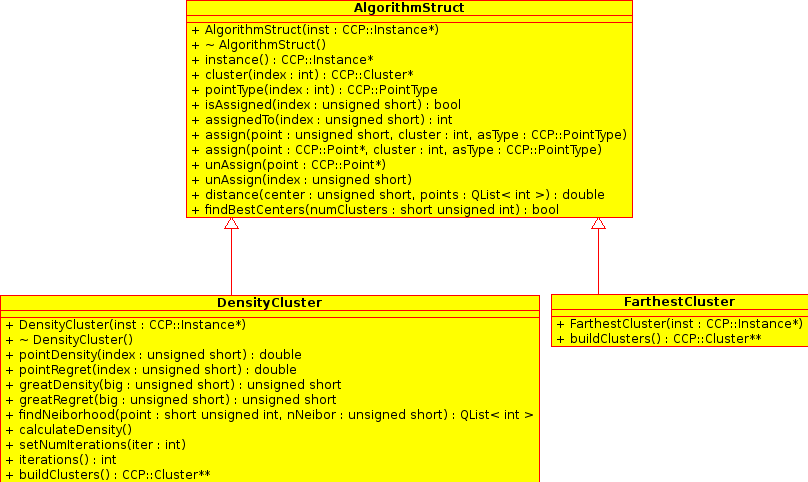
\includegraphics[bb=0 0 701 418, scale=0.6]{../TCC-I/imagens/Algorthms.png}
%  % Algorthms.png: 808x482 pixel, 83dpi, 24.72x14.75 cm, bb=0 0 701 418
% \caption{Classes dos algoritmos das heur�sticas de constru��o}
%
% \end{figure}
% %
% % \begin{figure}
% % \begin{center}
% % 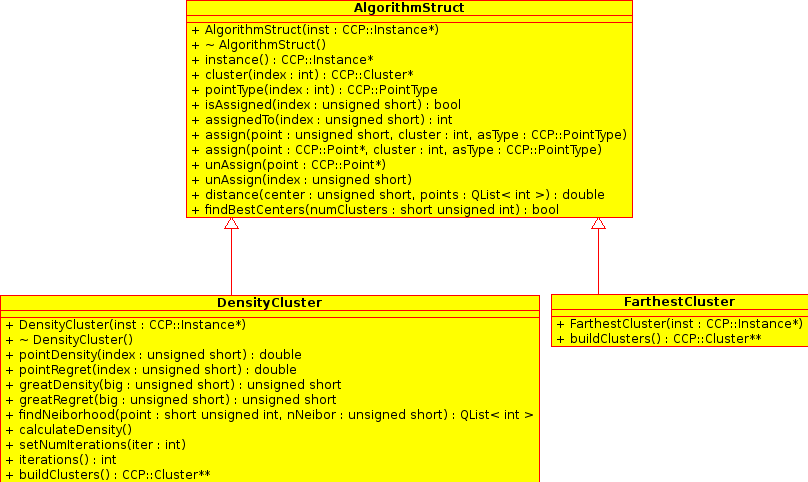
\includegraphics[scale=0.5]{../TCC-I/imagens/Algorthms.png}
% %
% % \end{center}
% % \end{figure}
%
%
% % \begin{landscape}
%
%
% \chapter*{Anexo B: Associa��o dos M�dulos}
% \renewcommand{\thefigure}{B.\arabic{figure}}
% %
% % 
\tikzset{
  arrow/.style={-stealth', line width=0.5pt},
  every picture/.append style={line width=1pt},
}

\tiny {

\enlargethispage{100cm}
% Start of code
% \begin{tikzpicture}[anchor=mid,>=latex',join=bevel,]
\begin{tikzpicture}[>=latex',join=bevel,scale=0.65]
  \pgfsetlinewidth{1bp}
%%
\pgfsetcolor{black}
  % Edge: node0 -> node4
  \draw [->] (130.06bp,219.43bp) .. controls (125.48bp,210.75bp) and (119.51bp,199.45bp)  .. (109.32bp,180.13bp);
  % Edge: node9 -> node12
  \draw [->] (716.02bp,147.39bp) .. controls (712.23bp,146.19bp) and (708.43bp,145.04bp)  .. (704.75bp,144bp) .. controls (632.92bp,123.76bp) and (612.69bp,127.83bp)  .. (540.75bp,108bp) .. controls (537.36bp,107.07bp) and (533.87bp,106.04bp)  .. (520.57bp,101.88bp);
  % Edge: node0 -> node11
  \draw [->] (108.83bp,226.23bp) .. controls (86.415bp,218.52bp) and (56.87bp,204.27bp)  .. (42.75bp,180bp) .. controls (31.694bp,161bp) and (36.774bp,136.1bp)  .. (47.572bp,107.83bp);
  % Edge: node6 -> node1
  \draw [->] (392.12bp,147.43bp) .. controls (390.6bp,139.01bp) and (388.64bp,128.14bp)  .. (385.02bp,108.13bp);
  % Edge: node9 -> node3
  \draw [->] (730.64bp,147.43bp) .. controls (710.16bp,136bp) and (681.55bp,120.03bp)  .. (650.79bp,102.86bp);
  % Edge: node8 -> node2
  \draw [->] (661.03bp,147.43bp) .. controls (677.35bp,137.64bp) and (699.21bp,124.52bp)  .. (726.54bp,108.13bp);
  % Edge: node5 -> node1
  \draw [->] (288.43bp,147.43bp) .. controls (304.26bp,137.68bp) and (325.46bp,124.64bp)  .. (352.29bp,108.13bp);
  % Edge: node2 -> node10
  \draw [->] (723.61bp,74.684bp) .. controls (720.65bp,73.658bp) and (717.67bp,72.741bp)  .. (714.75bp,72bp) .. controls (615.37bp,46.802bp) and (311.96bp,27.968bp)  .. (174.49bp,20.41bp);
  % Edge: node0 -> node1
  \draw [->] (143.2bp,219.19bp) .. controls (151.34bp,199.15bp) and (168.56bp,163.65bp)  .. (194.75bp,144bp) .. controls (234.16bp,114.43bp) and (289.34bp,101.03bp)  .. (339.68bp,93.545bp);
  % Edge: node5 -> node12
  \draw [->] (310.78bp,147.35bp) .. controls (344.57bp,136.56bp) and (391.55bp,121.49bp)  .. (432.75bp,108bp) .. controls (435.9bp,106.97bp) and (439.14bp,105.9bp)  .. (452.2bp,101.58bp);
  % Edge: node9 -> node2
  \draw [->] (756.75bp,147.43bp) .. controls (756.75bp,139.1bp) and (756.75bp,128.37bp)  .. (756.75bp,108.13bp);
  % Edge: node4 -> node1
  \draw [->] (147.76bp,147.85bp) .. controls (152.48bp,146.52bp) and (157.2bp,145.22bp)  .. (161.75bp,144bp) .. controls (218.97bp,128.68bp) and (285.01bp,112.7bp)  .. (339.44bp,99.83bp);
  % Edge: node8 -> node3
  \draw [->] (634.93bp,147.43bp) .. controls (633.86bp,138.89bp) and (632.48bp,127.82bp)  .. (629.95bp,107.6bp);
  % Edge: node6 -> node12
  \draw [->] (413.37bp,147.43bp) .. controls (426.18bp,137.4bp) and (443.46bp,123.88bp)  .. (466.24bp,106.05bp);
  % Edge: node7 -> node3
  \draw [->] (535.22bp,147.43bp) .. controls (553.25bp,136.24bp) and (578.27bp,120.71bp)  .. (606.27bp,103.33bp);
  % Edge: node6 -> node3
  \draw [->] (441.9bp,147.43bp) .. controls (483.67bp,134.52bp) and (544.13bp,115.84bp)  .. (594.23bp,100.36bp);
  % Edge: node4 -> node10
  \draw [->] (103.3bp,143.76bp) .. controls (108.09bp,119.09bp) and (116.69bp,74.86bp)  .. (124.23bp,36.09bp);
  % Edge: node0 -> node2
  \draw [->] (166.67bp,232.82bp) .. controls (294.44bp,227.45bp) and (803bp,204.6bp)  .. (825.75bp,180bp) .. controls (845.2bp,158.96bp) and (820.23bp,132.75bp)  .. (786.59bp,108.02bp);
  % Edge: node5 -> node3
  \draw [->] (320.06bp,147.35bp) .. controls (325.01bp,146.17bp) and (329.97bp,145.03bp)  .. (334.75bp,144bp) .. controls (425.61bp,124.41bp) and (449.45bp,125.42bp)  .. (540.75bp,108bp) .. controls (552.59bp,105.74bp) and (565.3bp,103.19bp)  .. (587.08bp,98.686bp);
  % Edge: node9 -> node1
  \draw [->] (717.25bp,147.4bp) .. controls (713.06bp,146.14bp) and (708.84bp,144.97bp)  .. (704.75bp,144bp) .. controls (589.21bp,116.65bp) and (553.22bp,135.4bp)  .. (423.85bp,105.62bp);
  % Edge: node7 -> node2
  \draw [->] (557.1bp,147.39bp) .. controls (561.03bp,146.21bp) and (564.95bp,145.07bp)  .. (568.75bp,144bp) .. controls (630.08bp,126.78bp) and (649.56bp,128.97bp)  .. (723.47bp,104.84bp);
  % Edge: node7 -> node12
  \draw [->] (506.69bp,147.43bp) .. controls (503.72bp,138.86bp) and (499.86bp,127.75bp)  .. (492.95bp,107.86bp);
  % Edge: node4 -> node11
  \draw [->] (88.899bp,143.83bp) .. controls (83.973bp,135.58bp) and (78.049bp,125.66bp)  .. (67.448bp,107.91bp);
  % Edge: node0 -> node3
  \draw [->] (166.8bp,232.75bp) .. controls (292.79bp,227.2bp) and (786.63bp,203.97bp)  .. (808.75bp,180bp) .. controls (819.6bp,168.24bp) and (818.31bp,156.83bp)  .. (808.75bp,144bp) .. controls (800.64bp,133.12bp) and (727.4bp,113.75bp)  .. (666.77bp,99.032bp);
  % Edge: node8 -> node1
  \draw [->] (581.63bp,147.41bp) .. controls (530.71bp,133.94bp) and (459.89bp,115.19bp)  .. (423.96bp,105.19bp);
  % Edge: node8 -> node12
  \draw [->] (606.39bp,147.43bp) .. controls (582.94bp,136.17bp) and (550.32bp,120.52bp)  .. (515.79bp,103.94bp);
  % Edge: node0 -> node10
  \draw [->] (108.77bp,225.48bp) .. controls (85.409bp,217.26bp) and (53.194bp,202.69bp)  .. (32.75bp,180bp) .. controls (9.7676bp,154.49bp) and (11.08bp,141.75bp)  .. (4.7496bp,108bp) .. controls (1.7995bp,92.274bp) and (-3.9994bp,85.396bp)  .. (4.7496bp,72bp) .. controls (20.241bp,48.28bp) and (48.728bp,34.912bp)  .. (84.051bp,24.816bp);
  % Edge: node7 -> node1
  \draw [->] (485.44bp,147.43bp) .. controls (467.6bp,137.55bp) and (443.66bp,124.29bp)  .. (414.48bp,108.13bp);
  % Node: node11
\begin{scope}
  \definecolor{strokecol}{rgb}{0.0,0.0,0.0};
  \pgfsetstrokecolor{strokecol}
  \draw (57bp,90bp) ellipse (43bp and 18bp);
  \draw (56.75bp,90bp) node {libQtGui.so};
\end{scope}
  % Node: node10
\begin{scope}
  \definecolor{strokecol}{rgb}{0.0,0.0,0.0};
  \pgfsetstrokecolor{strokecol}
  \draw (128bp,18bp) ellipse (47bp and 18bp);
  \draw (127.75bp,18bp) node {libQtCore.so};
\end{scope}
  % Node: node12
\begin{scope}
  \definecolor{strokecol}{rgb}{0.0,0.0,0.0};
  \pgfsetstrokecolor{strokecol}
  \draw (487bp,90bp) ellipse (45bp and 18bp);
  \draw (486.75bp,90bp) node {libQtTest.so};
\end{scope}
  % Node: node9
\begin{scope}
  \definecolor{strokecol}{rgb}{0.0,0.0,0.0};
  \pgfsetstrokecolor{strokecol}
  \draw (800bp,168bp) -- (757bp,180bp) -- (714bp,168bp) -- (714bp,147bp) -- (800bp,147bp) -- cycle;
  \draw (756.75bp,162bp) node {CCPTest};
\end{scope}
  % Node: node8
\begin{scope}
  \definecolor{strokecol}{rgb}{0.0,0.0,0.0};
  \pgfsetstrokecolor{strokecol}
  \draw (696bp,168bp) -- (637bp,180bp) -- (578bp,168bp) -- (578bp,147bp) -- (696bp,147bp) -- cycle;
  \draw (636.75bp,162bp) node {CCPSolution};
\end{scope}
  % Node: node1
\begin{scope}
  \definecolor{strokecol}{rgb}{0.0,0.0,0.0};
  \pgfsetstrokecolor{strokecol}
  \draw (424bp,108bp) -- (340bp,108bp) -- (340bp,72bp) -- (424bp,72bp) -- cycle;
  \draw (381.75bp,90bp) node {CCPModelLib};
\end{scope}
  % Node: node0
\begin{scope}
  \definecolor{strokecol}{rgb}{0.0,0.0,0.0};
  \pgfsetstrokecolor{strokecol}
  \draw (167bp,240bp) -- (138bp,252bp) -- (109bp,240bp) -- (109bp,219bp) -- (167bp,219bp) -- cycle;
  \draw (137.75bp,234bp) node {CCP};
\end{scope}
  % Node: node3
\begin{scope}
  \definecolor{strokecol}{rgb}{0.0,0.0,0.0};
  \pgfsetstrokecolor{strokecol}
  \draw (628bp,108bp) -- (550bp,90bp) -- (628bp,72bp) -- (706bp,90bp) -- cycle;
  \draw (627.75bp,90bp) node {CCPAlgorithms};
\end{scope}
  % Node: node2
\begin{scope}
  \definecolor{strokecol}{rgb}{0.0,0.0,0.0};
  \pgfsetstrokecolor{strokecol}
  \draw (790bp,108bp) -- (724bp,108bp) -- (724bp,72bp) -- (790bp,72bp) -- cycle;
  \draw (756.75bp,90bp) node {CCPIOLib};
\end{scope}
  % Node: node5
\begin{scope}
  \definecolor{strokecol}{rgb}{0.0,0.0,0.0};
  \pgfsetstrokecolor{strokecol}
  \draw (326bp,168bp) -- (265bp,180bp) -- (204bp,168bp) -- (204bp,147bp) -- (326bp,147bp) -- cycle;
  \draw (264.75bp,162bp) node {CCPDistance};
\end{scope}
  % Node: node4
\begin{scope}
  \definecolor{strokecol}{rgb}{0.0,0.0,0.0};
  \pgfsetstrokecolor{strokecol}
  \draw (148bp,180bp) -- (52bp,180bp) -- (52bp,144bp) -- (148bp,144bp) -- cycle;
  \draw (99.75bp,162bp) node {CCPClusterView};
\end{scope}
  % Node: node7
\begin{scope}
  \definecolor{strokecol}{rgb}{0.0,0.0,0.0};
  \pgfsetstrokecolor{strokecol}
  \draw (560bp,168bp) -- (512bp,180bp) -- (464bp,168bp) -- (464bp,147bp) -- (560bp,147bp) -- cycle;
  \draw (511.75bp,162bp) node {CCPRead};
\end{scope}
  % Node: node6
\begin{scope}
  \definecolor{strokecol}{rgb}{0.0,0.0,0.0};
  \pgfsetstrokecolor{strokecol}
  \draw (446bp,168bp) -- (395bp,180bp) -- (344bp,168bp) -- (344bp,147bp) -- (446bp,147bp) -- cycle;
  \draw (394.75bp,162bp) node {CCPModel};
\end{scope}
%
\end{tikzpicture}
% End of code

}
% \begin{figure}[ht]
%  \centering
%  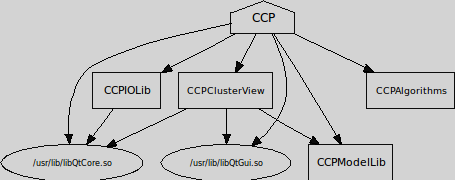
\includegraphics[bb=0 0 341 135]{./images/Modules.png}
%  % Modules.png: 455x180 pixel, 96dpi, 12.04x4.76 cm, bb=0 0 341 135
%
% \caption{Bibliotecas que fazem parte do sistema.}
%
% \end{figure}


% \end{landscape}



\end{document}



